\documentclass{article}
\usepackage[T1]{fontenc}
\usepackage{tgschola}
\usepackage[a4paper, total={6in, 8in}, margin=2cm]{geometry}
\usepackage{lipsum}
\usepackage{fancyhdr}
\usepackage{lastpage}
\setlength{\headheight}{48.2pt}
\usepackage{boxedminipage}
\usepackage{graphicx}
\usepackage[usestackEOL]{stackengine}
\graphicspath{ {./imagenes/} }
\pagestyle{fancy}
\usepackage{enumitem}
\usepackage[most]{tcolorbox}
\usepackage[option ]{askmaps}
\usepackage{circuitikz}
\usepackage{float}
\usepackage{adjustbox}
\usepackage{amsmath}
\usepackage{array}
\usepackage{multirow}
\usepackage{geometry}
\usepackage{booktabs}
\usepackage{tikz-timing}
\usepackage{url}

%%Modificar los siguientes valores segun la materia/tp
\newcommand{\Titulo}{Lenguajes Descriptivos de Hardware}
\newcommand{\Subtitulo}{Guía de Trabajos Prácticos}
\newcommand{\Version}{Versión 261C.01}
\newcommand{\Carrera}{INGENIERÍA EN ELECTRÓNICA}
\newcommand{\Asignatura}{3718 - Lenguajes Descriptivos de Hardware}
\newcommand{\Tema}{Diseño Sincrónico de Circuitos Digitales}
\newcommand{\Unidad}{1.0 - 4.0}
\newcommand{\Objetivo}{Repasar los fundamentos de los circuitos digitales, entender el diseño y funcionamiento de los circuitos lógicos programables (FPGAs), diseñar circuitos sincrónicos utilizando síntesis mediante lenguajes descriptivos como Verilog}
\newcommand{\TiempoResolucion}{Cuatrimestral}
\newcommand{\Metodologia}{Simulador Logisim-Evolution; Xilinx Vivado; Xilinx Vitis}
\newcommand{\Entrega}{No obligatoria, desarrollo en laboratorio}


\fancyhead[L]{\framebox(128,64){\includegraphics[scale=0.18]{diit}}}
\fancyhead[C]{\framebox(224,64){\Longstack{\textbf{\Titulo}\\\textbf{\Subtitulo}\\Pág. \thepage\ de \pageref{LastPage}}}}
\fancyhead[R]{\framebox(128,64){\includegraphics[scale=0.055]{logo}}}
\renewcommand{\headrulewidth}{0.0pt}
\renewcommand{\footrulewidth}{0pt}




\begin{document}
	
	
	\centering\LARGE{\textbf{\Version}}
	\large
	\\
	\begin{center}
		\begin{tabular}{|p{15cm}|} % 'l' for left-aligned, 'p' for paragraph with specified width
			
			\hline
			\rule{0pt}{15pt}
			\textbf{Carrera: \Carrera} \\
			\hline
			\rule{0pt}{15pt}
			\textbf{Asignatura:}  \Asignatura \\
			\hline
			\rule{0pt}{15pt}
			\textbf{Tema:}  \Tema \\
			\hline
			\rule{0pt}{15pt}
			\textbf{Unidad:}  \Unidad \\
			\hline
			\rule{0pt}{15pt}
			\textbf{Objetivo:} \Objetivo \\
			\hline
			\rule{0pt}{15pt}
			\textbf{Competencias a desarrollar:} 
			\begin{itemize}
				\item Concepción, diseño y desarrollo de proyectos de ingeniería en electrónica.
				\item Gestión, planificación, ejecución y control de proyectos de ingeniería en electrónica.
				\item Utilización de técnicas y herramientas de aplicación en la ingeniería en electrónica.
				\item Generación de desarrollos tecnológicos y/o innovaciones tecnológicas.
				\item Desarrollo de una actitud profesional emprendedora.
				\item Aprendizaje continuo
				\item Actuación profesional ética y responsable.
				\item Comunicación efectiva.
				\item Desempeño en equipos de trabajo.
				\item Identificación, formulación y resolución de problemas de ingeniería en electrónica
			\end{itemize} \\
			\hline
			\rule{0pt}{15pt}
			\textbf{Descripción de la actividad:} 
			\begin{enumerate}
				\item  Tiempo estimado de resolución: \TiempoResolucion
				\item Metodología: \Metodologia
				\item Forma de entrega: \Entrega
				\item Metodología de corrección y feedback al alumno: Presencial y por Miel.
			\end{enumerate} \\
			\hline
		\end{tabular}
	\end{center}
	
	\clearpage
	
		\section*{A- Repaso}
		\begin{tcolorbox}[enhanced,attach boxed title to top center={yshift=-3mm,yshifttext=-1mm},
			colback=black!5!white,colframe=white!75!black,colbacktitle=red!80!black,
			title= Consejo , fonttitle=\bfseries,
			boxed title style={size=small,colframe=white,colback=black} ]
			Los siguientes ejercicios requieren repasar los temas vistos en las materias previas de técnicas digitales. Dejamos en MIeL una lista de reproducción con videos de repaso sobre estos temas.  
		\end{tcolorbox}
	\begin{enumerate}[label=\textbf{A.\arabic*}]
		\item Dada la siguiente tabla de verdad para la función F(A,B,C,D)\\
		\begin{tabular}{cccc|c}
			A & B & C & D & F \\
			\hline
			0 & 0 & 0 & 0 & 0 \\
			0 & 0 & 0 & 1 & 0 \\
			0 & 0 & 1 & 0 & 0 \\
			0 & 0 & 1 & 1 & 0 \\
			0 & 1 & 0 & 0 & 1 \\
			0 & 1 & 0 & 1 & 1 \\
			0 & 1 & 1 & 0 & 1 \\
			0 & 1 & 1 & 1 & X \\
			1 & 0 & 0 & 0 & 0 \\
			1 & 0 & 0 & 1 & 0 \\
			1 & 0 & 1 & 0 & 0 \\
			1 & 0 & 1 & 1 & 0 \\
			1 & 1 & 0 & 0 & 1 \\
			1 & 1 & 0 & 1 & 0 \\
			1 & 1 & 1 & 0 & 1 \\
			1 & 1 & 1 & 1 & 0 \\
		\end{tabular}
		 \begin{enumerate}
		 	\item Escriba la función F(A,B,C,D) en primera forma canónica (suma de productos).\\ \textbf{ F(A,B,C,D)= }\\
		 	\item Escriba la función F(A,B,C,D) en segunda forma canónica (producto de sumas).\\ \textbf{ F(A,B,C,D)= }\\
		 	\item Simplifique F (minitérminos) utilizando el mapa de Karnaugh y luego implemente el circuito simplificado utilizando solo compuertas NAND.\\ \askmapiv{F}{CDAB}{}{}{}
		 	\item Implemente el circuito utilizando un MUX de 4 entradas de selección.\\
		 	\resizebox{!}{6cm} {
			\begin{tikzpicture}[x=1pt,y=-1pt,line cap=rect]
				\def\logisimfontA#1{\fontfamily{cmr}{#1}} % Replaced by logisim, original font was "SansSerif"
				\def\logisimfontB#1{\fontfamily{cmtt}{#1}} % Replaced by logisim, original font was "Monospaced"
				\definecolor{custcol_0_0_ff}{RGB}{0, 0, 255}
				\definecolor{custcol_0_0_0}{RGB}{0, 0, 0}
				\definecolor{custcol_ff_ff_ff}{RGB}{255, 255, 255}
				\definecolor{custcol_80_80_80}{RGB}{128, 128, 128}
				\definecolor{custcol_c0_c0_c0}{RGB}{192, 192, 192}
				\definecolor{custcol_28_28_ff}{RGB}{40, 40, 255}
				\draw [line width=3.0pt, custcol_28_28_ff ]  (35.0,65.0) -- (95.0,65.0) ;
				\draw [line width=3.0pt, custcol_28_28_ff ]  (35.0,115.0) -- (95.0,115.0) ;
				\draw [line width=3.0pt, custcol_28_28_ff ]  (45.0,55.0) -- (95.0,55.0) ;
				\draw [line width=3.0pt, custcol_28_28_ff ]  (45.0,125.0) -- (95.0,125.0) ;
				\draw [line width=4.0pt, custcol_0_0_0 ]  (115.0,175.0) -- (115.0,205.0) ;
				\draw [line width=3.0pt, custcol_28_28_ff ]  (55.0,45.0) -- (95.0,45.0) ;
				\draw [line width=3.0pt, custcol_28_28_ff ]  (55.0,135.0) -- (95.0,135.0) ;
				\draw [line width=3.0pt, custcol_28_28_ff ]  (65.0,35.0) -- (95.0,35.0) ;
				\draw [line width=3.0pt, custcol_28_28_ff ]  (65.0,145.0) -- (95.0,145.0) ;
				\draw [line width=3.0pt, custcol_28_28_ff ]  (5.0,95.0) -- (95.0,95.0) ;
				\draw [line width=3.0pt, custcol_28_28_ff ]  (135.0,95.0) -- (155.0,95.0) ;
				\draw [line width=3.0pt, custcol_28_28_ff ]  (75.0,25.0) -- (95.0,25.0) ;
				\draw [line width=3.0pt, custcol_28_28_ff ]  (75.0,155.0) -- (95.0,155.0) ;
				\draw [line width=3.0pt, custcol_28_28_ff ]  (15.0,85.0) -- (95.0,85.0) ;
				\draw [line width=3.0pt, custcol_28_28_ff ]  (15.0,105.0) -- (95.0,105.0) ;
				\draw [line width=3.0pt, custcol_28_28_ff ]  (85.0,15.0) -- (95.0,15.0) ;
				\draw [line width=3.0pt, custcol_28_28_ff ]  (85.0,165.0) -- (95.0,165.0) ;
				\draw [line width=3.0pt, custcol_28_28_ff ]  (25.0,75.0) -- (95.0,75.0) ;
				\fill [line width=1.0pt, custcol_c0_c0_c0]  (115.0,165.0) ellipse (3.0 and 3.0 );
				\logisimfontA{\fontsize{12pt}{12pt}\selectfont\node[inner sep=0, outer sep=0, custcol_80_80_80, anchor=base west] at  (98.0,20.0)  {0};}
				\draw [line width=2.0pt, custcol_0_0_0 ]  (95.0,5.0) -- (135.0,25.0) -- (135.0,165.0) -- (95.0,185.0) -- cycle;
				\logisimfontA{\fontsize{12pt}{12pt}\selectfont\node[inner sep=0, outer sep=0, custcol_0_0_0, anchor=base west] at  (102.0,101.0)  {MUX};}
				\fill [line width=2.0pt, custcol_28_28_ff]  (95.0,15.0) ellipse (2.0 and 2.0 );
				\fill [line width=2.0pt, custcol_28_28_ff]  (95.0,25.0) ellipse (2.0 and 2.0 );
				\fill [line width=2.0pt, custcol_28_28_ff]  (95.0,35.0) ellipse (2.0 and 2.0 );
				\fill [line width=2.0pt, custcol_28_28_ff]  (95.0,45.0) ellipse (2.0 and 2.0 );
				\fill [line width=2.0pt, custcol_28_28_ff]  (95.0,55.0) ellipse (2.0 and 2.0 );
				\fill [line width=2.0pt, custcol_28_28_ff]  (95.0,65.0) ellipse (2.0 and 2.0 );
				\fill [line width=2.0pt, custcol_28_28_ff]  (95.0,75.0) ellipse (2.0 and 2.0 );
				\fill [line width=2.0pt, custcol_28_28_ff]  (95.0,85.0) ellipse (2.0 and 2.0 );
				\fill [line width=2.0pt, custcol_28_28_ff]  (95.0,95.0) ellipse (2.0 and 2.0 );
				\fill [line width=2.0pt, custcol_28_28_ff]  (95.0,105.0) ellipse (2.0 and 2.0 );
				\fill [line width=2.0pt, custcol_28_28_ff]  (95.0,115.0) ellipse (2.0 and 2.0 );
				\fill [line width=2.0pt, custcol_28_28_ff]  (95.0,125.0) ellipse (2.0 and 2.0 );
				\fill [line width=2.0pt, custcol_28_28_ff]  (95.0,135.0) ellipse (2.0 and 2.0 );
				\fill [line width=2.0pt, custcol_28_28_ff]  (95.0,145.0) ellipse (2.0 and 2.0 );
				\fill [line width=2.0pt, custcol_28_28_ff]  (95.0,155.0) ellipse (2.0 and 2.0 );
				\fill [line width=2.0pt, custcol_28_28_ff]  (95.0,165.0) ellipse (2.0 and 2.0 );
				\fill [line width=2.0pt, custcol_0_0_0]  (115.0,175.0) ellipse (2.0 and 2.0 );
				\fill [line width=2.0pt, custcol_28_28_ff]  (135.0,95.0) ellipse (2.0 and 2.0 );
				\draw [line width=3.0pt, custcol_28_28_ff ]  (159.0,95.0) -- (156.0,95.0) ;
				\draw [line width=2.0pt, custcol_0_0_0 ]  (185.0,86.0) -- (195.0,95.0) -- (185.0,104.0) -- (161.0,104.0) -- (161.0,86.0) -- cycle;
				\logisimfontB{\fontsize{12pt}{12pt}\selectfont\node[inner sep=0, outer sep=0, custcol_0_0_ff, anchor=base west] at  (180.0,102.0)  {b};}
				\logisimfontB{\fontsize{12pt}{12pt}\selectfont\node[inner sep=0, outer sep=0, custcol_0_0_0, anchor=base west] at  (172.0,98.0)  {U};}
				\logisimfontA{\fontsize{16pt}{16pt}\fontseries{bx}\selectfont\node[inner sep=0, outer sep=0, custcol_0_0_ff, anchor=base west] at  (197.0,102.0)  {F};}
				\fill [line width=2.0pt, custcol_28_28_ff]  (155.0,95.0) ellipse (2.0 and 2.0 );
				\draw [line width=3.0pt, custcol_28_28_ff ]  (105.0,245.0) -- (105.0,225.0) -- (105.0,211.0) ;
				\draw [line width=3.0pt, custcol_28_28_ff ]  (85.0,245.0) -- (85.0,225.0) -- (85.0,211.0) ;
				\draw [line width=3.0pt, custcol_28_28_ff ]  (65.0,245.0) -- (65.0,225.0) -- (65.0,211.0) ;
				\draw [line width=3.0pt, custcol_28_28_ff ]  (45.0,245.0) -- (45.0,225.0) -- (45.0,211.0) ;
				\draw [line width=5.0pt, custcol_0_0_0 ]  (46.0,211.0) -- (109.0,211.0) -- (114.0,206.0) ;
				\logisimfontA{\fontsize{7pt}{7pt}\selectfont\node[inner sep=0, outer sep=0, custcol_0_0_0, anchor=base west, rotate=-90.0] at  (108.0,214.0)  {0};}
				\logisimfontA{\fontsize{7pt}{7pt}\selectfont\node[inner sep=0, outer sep=0, custcol_0_0_0, anchor=base west, rotate=-90.0] at  (88.0,214.0)  {1};}
				\logisimfontA{\fontsize{7pt}{7pt}\selectfont\node[inner sep=0, outer sep=0, custcol_0_0_0, anchor=base west, rotate=-90.0] at  (68.0,214.0)  {2};}
				\logisimfontA{\fontsize{7pt}{7pt}\selectfont\node[inner sep=0, outer sep=0, custcol_0_0_0, anchor=base west, rotate=-90.0] at  (48.0,214.0)  {3};}
				\fill [line width=5.0pt, custcol_0_0_0]  (115.0,205.0) ellipse (2.0 and 2.0 );
				\fill [line width=5.0pt, custcol_28_28_ff]  (105.0,225.0) ellipse (2.0 and 2.0 );
				\fill [line width=5.0pt, custcol_28_28_ff]  (85.0,225.0) ellipse (2.0 and 2.0 );
				\fill [line width=5.0pt, custcol_28_28_ff]  (65.0,225.0) ellipse (2.0 and 2.0 );
				\fill [line width=5.0pt, custcol_28_28_ff]  (45.0,225.0) ellipse (2.0 and 2.0 );
				\logisimfontA{\fontsize{16pt}{16pt}\fontseries{bx}\selectfont\node[inner sep=0, outer sep=0, custcol_0_0_0, anchor=base west] at  (39.0,265.0)  {A};}
				\draw [line width=2.0pt, custcol_0_0_0 ]  (36.0,249.0) -- (45.0,245.0) -- (54.0,249.0) -- (54.0,272.0) -- (36.0,272.0) -- cycle;
				\fill [line width=2.0pt, custcol_28_28_ff]  (45.0,245.0) ellipse (2.0 and 2.0 );
				\logisimfontA{\fontsize{16pt}{16pt}\fontseries{bx}\selectfont\node[inner sep=0, outer sep=0, custcol_0_0_0, anchor=base west] at  (59.0,265.0)  {B};}
				\draw [line width=2.0pt, custcol_0_0_0 ]  (56.0,249.0) -- (65.0,245.0) -- (74.0,249.0) -- (74.0,272.0) -- (56.0,272.0) -- cycle;
				\fill [line width=2.0pt, custcol_28_28_ff]  (65.0,245.0) ellipse (2.0 and 2.0 );
				\logisimfontA{\fontsize{16pt}{16pt}\fontseries{bx}\selectfont\node[inner sep=0, outer sep=0, custcol_0_0_0, anchor=base west] at  (79.0,265.0)  {C};}
				\draw [line width=2.0pt, custcol_0_0_0 ]  (76.0,249.0) -- (85.0,245.0) -- (94.0,249.0) -- (94.0,272.0) -- (76.0,272.0) -- cycle;
				\fill [line width=2.0pt, custcol_28_28_ff]  (85.0,245.0) ellipse (2.0 and 2.0 );
				\logisimfontA{\fontsize{16pt}{16pt}\fontseries{bx}\selectfont\node[inner sep=0, outer sep=0, custcol_0_0_0, anchor=base west] at  (99.0,265.0)  {D};}
				\draw [line width=2.0pt, custcol_0_0_0 ]  (96.0,249.0) -- (105.0,245.0) -- (115.0,249.0) -- (115.0,272.0) -- (96.0,272.0) -- cycle;
				\fill [line width=2.0pt, custcol_28_28_ff]  (105.0,245.0) ellipse (2.0 and 2.0 );
				
			\end{tikzpicture}
		}
		
		 
		 \item Para los dos circuitos previos (simplificado y MUX) simule ambos en logisim-evolution y verifique que la salida F genera los mismos valores en todos los casos.
		 \end{enumerate}
		\item Utilizando logisim-evolution diseñe un conversor BCD a 7 segmentos. Puede implementar el mismo de la forma que crea mas conveniente (simplificando 7 funciones, con MUXes, con una ROM de LookUp Table, etc). \\
	\begin{tikzpicture}[x=1pt,y=-1pt,line cap=rect]
		\def\logisimfontA#1{\fontfamily{cmr}{#1}} % Replaced by logisim, original font was "SansSerif"
		\def\logisimfontB#1{\fontfamily{Dialog}{#1}}
		\def\logisimfontC#1{\fontfamily{cmtt}{#1}} % Replaced by logisim, original font was "Monospaced"
		\definecolor{custcol_0_0_ff}{RGB}{0, 0, 255}
		\definecolor{custcol_0_64_0}{RGB}{0, 100, 0}
		\definecolor{custcol_0_0_0}{RGB}{0, 0, 0}
		\definecolor{custcol_0_d2_0}{RGB}{0, 210, 0}
		\definecolor{custcol_40_40_40}{RGB}{64, 64, 64}
		\definecolor{custcol_ff_ff_ff}{RGB}{255, 255, 255}
		\definecolor{custcol_dc_dc_dc}{RGB}{220, 220, 220}
		\definecolor{custcol_f0_0_0}{RGB}{240, 0, 0}
		\definecolor{custcol_28_28_ff}{RGB}{40, 40, 255}
		\draw [line width=4.0pt, custcol_0_0_0 ]  (344.0,135.0) -- (354.0,135.0) ;
		\fill [line width=1.0pt, custcol_0_0_0 ]  (124.0,133.0) rectangle (134.0,137.0) ;
		\logisimfontB{\fontsize{12pt}{12pt}\selectfont\node[inner sep=0, outer sep=0, custcol_40_40_40, anchor=base west] at  (139.0,139.0)  {BCD};}
		\fill [line width=1.0pt, custcol_0_0_0 ]  (334.0,133.0) rectangle (344.0,137.0) ;
		\logisimfontB{\fontsize{12pt}{12pt}\selectfont\node[inner sep=0, outer sep=0, custcol_40_40_40, anchor=base west] at  (273.0,139.0)  {SieteSeg};}
		\fill [line width=1.0pt, custcol_0_0_0 ]  (134.0,145.0) rectangle (334.0,165.0) ;
		\draw [line width=2.0pt, custcol_0_0_0 ]  (134.0,125.0) -- (333.0,125.0) ;
		\draw [line width=2.0pt, custcol_0_0_0 ]  (334.0,125.0) -- (334.0,164.0) ;
		\draw [line width=2.0pt, custcol_0_0_0 ]  (334.0,165.0) -- (135.0,165.0) ;
		\draw [line width=2.0pt, custcol_0_0_0 ]  (134.0,165.0) -- (134.0,126.0) ;
		\logisimfontB{\fontsize{14pt}{14pt}\fontseries{bx}\selectfont\node[inner sep=0, outer sep=0, custcol_ff_ff_ff, anchor=base west] at  (197.0,159.0)  {BCD7SEG};}
		\fill [line width=1.0pt, custcol_0_0_0]  (124.0,135.0) ellipse (2.0 and 2.0 );
		\fill [line width=1.0pt, custcol_0_0_0]  (344.0,135.0) ellipse (2.0 and 2.0 );
		\draw [line width=4.0pt, custcol_0_0_0 ]  (111.0,135.0) -- (114.0,135.0) -- (124.0,135.0) ;
		\draw [line width=2.0pt, custcol_0_0_0 ]  (99.0,144.0) -- (109.0,135.0) -- (99.0,126.0) -- (45.0,126.0) -- (45.0,144.0) -- cycle;
		\logisimfontC{\fontsize{12pt}{12pt}\selectfont\node[inner sep=0, outer sep=0, custcol_0_0_ff, anchor=base west] at  (94.0,142.0)  {b};}
		\fill [line width=2.0pt, custcol_0_d2_0]  (89.0,134.0) ellipse (4.5 and 7.0 );
		\logisimfontC{\fontsize{12pt}{12pt}\selectfont\node[inner sep=0, outer sep=0, custcol_ff_ff_ff, anchor=base west] at  (86.0,138.0)  {1};}
		\fill [line width=2.0pt, custcol_0_d2_0]  (79.0,134.0) ellipse (4.5 and 7.0 );
		\logisimfontC{\fontsize{12pt}{12pt}\selectfont\node[inner sep=0, outer sep=0, custcol_ff_ff_ff, anchor=base west] at  (76.0,138.0)  {1};}
		\fill [line width=2.0pt, custcol_0_d2_0]  (69.0,134.0) ellipse (4.5 and 7.0 );
		\logisimfontC{\fontsize{12pt}{12pt}\selectfont\node[inner sep=0, outer sep=0, custcol_ff_ff_ff, anchor=base west] at  (66.0,138.0)  {1};}
		\fill [line width=2.0pt, custcol_0_64_0]  (59.0,134.0) ellipse (4.5 and 7.0 );
		\logisimfontC{\fontsize{12pt}{12pt}\selectfont\node[inner sep=0, outer sep=0, custcol_ff_ff_ff, anchor=base west] at  (56.0,138.0)  {0};}
		\logisimfontA{\fontsize{16pt}{16pt}\fontseries{bx}\selectfont\node[inner sep=0, outer sep=0, custcol_0_0_ff, anchor=base west] at  (5.0,142.0)  {BCD};}
		\fill [line width=2.0pt, custcol_0_0_0]  (114.0,135.0) ellipse (2.0 and 2.0 );
		\draw [line width=3.0pt, custcol_0_d2_0 ]  (464.0,75.0) -- (464.0,5.0) -- (374.0,5.0) -- (360.0,5.0) ;
		\draw [line width=3.0pt, custcol_0_d2_0 ]  (474.0,75.0) -- (474.0,25.0) -- (374.0,25.0) -- (360.0,25.0) ;
		\draw [line width=3.0pt, custcol_0_d2_0 ]  (464.0,135.0) -- (464.0,145.0) -- (494.0,145.0) -- (494.0,45.0) -- (374.0,45.0) -- (360.0,45.0) ;
		\draw [line width=3.0pt, custcol_0_64_0 ]  (454.0,135.0) -- (454.0,165.0) -- (414.0,165.0) -- (414.0,65.0) -- (374.0,65.0) -- (360.0,65.0) ;
		\draw [line width=3.0pt, custcol_0_64_0 ]  (444.0,135.0) -- (444.0,145.0) -- (394.0,145.0) -- (394.0,85.0) -- (374.0,85.0) -- (360.0,85.0) ;
		\draw [line width=3.0pt, custcol_0_64_0 ]  (454.0,75.0) -- (454.0,65.0) -- (424.0,65.0) -- (424.0,105.0) -- (374.0,105.0) -- (360.0,105.0) ;
		\draw [line width=3.0pt, custcol_0_64_0 ]  (444.0,75.0) -- (444.0,55.0) -- (434.0,55.0) -- (434.0,125.0) -- (374.0,125.0) -- (360.0,125.0) ;
		\draw [line width=5.0pt, custcol_0_0_0 ]  (360.0,6.0) -- (360.0,129.0) -- (355.0,134.0) ;
		\logisimfontA{\fontsize{7pt}{7pt}\selectfont\node[inner sep=0, outer sep=0, custcol_0_0_0, anchor=base west] at  (363.0,12.0)  {0};}
		\logisimfontA{\fontsize{7pt}{7pt}\selectfont\node[inner sep=0, outer sep=0, custcol_0_0_0, anchor=base west] at  (363.0,32.0)  {1};}
		\logisimfontA{\fontsize{7pt}{7pt}\selectfont\node[inner sep=0, outer sep=0, custcol_0_0_0, anchor=base west] at  (363.0,52.0)  {2};}
		\logisimfontA{\fontsize{7pt}{7pt}\selectfont\node[inner sep=0, outer sep=0, custcol_0_0_0, anchor=base west] at  (363.0,72.0)  {3};}
		\logisimfontA{\fontsize{7pt}{7pt}\selectfont\node[inner sep=0, outer sep=0, custcol_0_0_0, anchor=base west] at  (363.0,92.0)  {4};}
		\logisimfontA{\fontsize{7pt}{7pt}\selectfont\node[inner sep=0, outer sep=0, custcol_0_0_0, anchor=base west] at  (363.0,112.0)  {5};}
		\logisimfontA{\fontsize{7pt}{7pt}\selectfont\node[inner sep=0, outer sep=0, custcol_0_0_0, anchor=base west] at  (363.0,132.0)  {6};}
		\fill [line width=5.0pt, custcol_0_0_0]  (354.0,135.0) ellipse (2.0 and 2.0 );
		\fill [line width=5.0pt, custcol_0_d2_0]  (374.0,5.0) ellipse (2.0 and 2.0 );
		\fill [line width=5.0pt, custcol_0_d2_0]  (374.0,25.0) ellipse (2.0 and 2.0 );
		\fill [line width=5.0pt, custcol_0_d2_0]  (374.0,45.0) ellipse (2.0 and 2.0 );
		\fill [line width=5.0pt, custcol_0_64_0]  (374.0,65.0) ellipse (2.0 and 2.0 );
		\fill [line width=5.0pt, custcol_0_64_0]  (374.0,85.0) ellipse (2.0 and 2.0 );
		\fill [line width=5.0pt, custcol_0_64_0]  (374.0,105.0) ellipse (2.0 and 2.0 );
		\fill [line width=5.0pt, custcol_0_64_0]  (374.0,125.0) ellipse (2.0 and 2.0 );
		\draw [line width=2.0pt, custcol_0_0_0 ]  (439.0,75.0) -- (478.0,75.0) ;
		\draw [line width=2.0pt, custcol_0_0_0 ]  (479.0,75.0) -- (479.0,134.0) ;
		\draw [line width=2.0pt, custcol_0_0_0 ]  (479.0,135.0) -- (440.0,135.0) ;
		\draw [line width=2.0pt, custcol_0_0_0 ]  (439.0,135.0) -- (439.0,76.0) ;
		\fill [line width=1.0pt, custcol_f0_0_0 ]  (447.0,83.0) rectangle (466.0,87.0) ;
		\fill [line width=1.0pt, custcol_f0_0_0 ]  (467.0,85.0) rectangle (471.0,104.0) ;
		\fill [line width=1.0pt, custcol_f0_0_0 ]  (467.0,105.0) rectangle (471.0,124.0) ;
		\fill [line width=1.0pt, custcol_dc_dc_dc ]  (447.0,122.0) rectangle (466.0,126.0) ;
		\fill [line width=1.0pt, custcol_dc_dc_dc ]  (442.0,105.0) rectangle (446.0,124.0) ;
		\fill [line width=1.0pt, custcol_dc_dc_dc ]  (442.0,85.0) rectangle (446.0,104.0) ;
		\fill [line width=1.0pt, custcol_dc_dc_dc ]  (447.0,103.0) rectangle (466.0,107.0) ;
		\fill [line width=1.0pt, custcol_dc_dc_dc]  (474.0,125.0) ellipse (2.5 and 2.5 );
		\fill [line width=1.0pt, custcol_0_d2_0]  (464.0,75.0) ellipse (2.0 and 2.0 );
		\fill [line width=1.0pt, custcol_0_d2_0]  (474.0,75.0) ellipse (2.0 and 2.0 );
		\fill [line width=1.0pt, custcol_0_d2_0]  (464.0,135.0) ellipse (2.0 and 2.0 );
		\fill [line width=1.0pt, custcol_0_64_0]  (454.0,135.0) ellipse (2.0 and 2.0 );
		\fill [line width=1.0pt, custcol_0_64_0]  (444.0,135.0) ellipse (2.0 and 2.0 );
		\fill [line width=1.0pt, custcol_0_64_0]  (454.0,75.0) ellipse (2.0 and 2.0 );
		\fill [line width=1.0pt, custcol_0_64_0]  (444.0,75.0) ellipse (2.0 and 2.0 );
		\fill [line width=1.0pt, custcol_28_28_ff]  (474.0,135.0) ellipse (2.0 and 2.0 );
	\end{tikzpicture}
		\item \label{latch} Utilizando 3 FlipFlops tipo D, implemente en logisim-evolution el siguiente registro Latch de 3 bits con entrada paralelo y salida paralelo.\\
		\begin{adjustbox}{width=\textwidth}
		\begin{tikzpicture}[x=1pt,y=-1pt,line cap=rect]
			\def\logisimfontA#1{\fontfamily{cmr}{#1}} % Replaced by logisim, original font was "SansSerif"
			\def\logisimfontB#1{\fontfamily{cmtt}{#1}} % Replaced by logisim, original font was "Monospaced"
			\definecolor{custcol_0_0_ff}{RGB}{0, 0, 255}
			\definecolor{custcol_0_64_0}{RGB}{0, 100, 0}
			\definecolor{custcol_0_0_0}{RGB}{0, 0, 0}
			\definecolor{custcol_0_d2_0}{RGB}{0, 210, 0}
			\definecolor{custcol_ff_ff_ff}{RGB}{255, 255, 255}
			\definecolor{custcol_80_80_80}{RGB}{128, 128, 128}
			\definecolor{custcol_28_28_ff}{RGB}{40, 40, 255}
			\draw [line width=4.0pt, custcol_0_0_0 ]  (495.0,185.0) -- (515.0,185.0) ;
			\draw [line width=3.0pt, custcol_0_64_0 ]  (155.0,115.0) -- (185.0,115.0) -- (185.0,145.0) -- (295.0,145.0) -- (405.0,145.0) -- (405.0,115.0) -- (415.0,115.0) ;
			\draw [line width=3.0pt, custcol_0_64_0 ]  (295.0,145.0) -- (295.0,115.0) -- (305.0,115.0) ;
			\fill [line width=3.0pt, custcol_0_64_0]  (295.0,145.0) ellipse (5.0 and 5.0 );
			\fill [line width=3.0pt, custcol_0_64_0]  (185.0,115.0) ellipse (5.0 and 5.0 );
			\draw [line width=2.0pt, custcol_0_0_0 ]  (195.0,65.0) -- (234.0,65.0) ;
			\draw [line width=2.0pt, custcol_0_0_0 ]  (235.0,65.0) -- (235.0,124.0) ;
			\draw [line width=2.0pt, custcol_0_0_0 ]  (235.0,125.0) -- (196.0,125.0) ;
			\draw [line width=2.0pt, custcol_0_0_0 ]  (195.0,125.0) -- (195.0,66.0) ;
			\fill [line width=2.0pt, custcol_0_64_0]  (215.0,95.0) ellipse (7.0 and 7.0 );
			\logisimfontA{\fontsize{12pt}{12pt}\selectfont\node[inner sep=0, outer sep=0, custcol_ff_ff_ff, anchor=base west] at  (211.0,99.0)  {0};}
			\fill [line width=2.0pt, custcol_28_28_ff]  (215.0,125.0) ellipse (2.0 and 2.0 );
			\logisimfontA{\fontsize{12pt}{12pt}\selectfont\node[inner sep=0, outer sep=0, custcol_80_80_80, anchor=base west] at  (211.0,122.0)  {R};}
			\fill [line width=2.0pt, custcol_28_28_ff]  (215.0,65.0) ellipse (2.0 and 2.0 );
			\logisimfontA{\fontsize{12pt}{12pt}\selectfont\node[inner sep=0, outer sep=0, custcol_80_80_80, anchor=base west] at  (211.0,80.0)  {S};}
			\draw [line width=3.0pt, custcol_0_0_0 ]  (185.0,75.0) -- (194.0,75.0) ;
			\fill [line width=3.0pt, custcol_0_64_0]  (185.0,75.0) ellipse (2.0 and 2.0 );
			\logisimfontA{\fontsize{12pt}{12pt}\selectfont\node[inner sep=0, outer sep=0, custcol_0_0_0, anchor=base west] at  (199.0,79.0)  {D};}
			\draw [line width=2.0pt, custcol_0_0_0 ]  (196.0,111.0) -- (203.0,115.0) -- (196.0,119.0) ;
			\draw [line width=2.0pt, custcol_0_0_0 ]  (185.0,115.0) -- (194.0,115.0) ;
			\fill [line width=2.0pt, custcol_0_64_0]  (185.0,115.0) ellipse (2.0 and 2.0 );
			\draw [line width=3.0pt, custcol_0_0_0 ]  (236.0,75.0) -- (245.0,75.0) ;
			\logisimfontA{\fontsize{12pt}{12pt}\selectfont\node[inner sep=0, outer sep=0, custcol_0_0_0, anchor=base west] at  (222.0,79.0)  {Q};}
			\fill [line width=3.0pt, custcol_0_64_0]  (245.0,75.0) ellipse (2.0 and 2.0 );
			\draw [line width=2.0pt, custcol_0_0_0]  (240.0,115.0) ellipse (5.0 and 5.0 );
			\fill [line width=2.0pt, custcol_0_d2_0]  (245.0,115.0) ellipse (2.0 and 2.0 );
			\draw [line width=2.0pt, custcol_0_0_0 ]  (315.0,65.0) -- (354.0,65.0) ;
			\draw [line width=2.0pt, custcol_0_0_0 ]  (355.0,65.0) -- (355.0,124.0) ;
			\draw [line width=2.0pt, custcol_0_0_0 ]  (355.0,125.0) -- (316.0,125.0) ;
			\draw [line width=2.0pt, custcol_0_0_0 ]  (315.0,125.0) -- (315.0,66.0) ;
			\fill [line width=2.0pt, custcol_0_64_0]  (335.0,95.0) ellipse (7.0 and 7.0 );
			\logisimfontA{\fontsize{12pt}{12pt}\selectfont\node[inner sep=0, outer sep=0, custcol_ff_ff_ff, anchor=base west] at  (331.0,99.0)  {0};}
			\fill [line width=2.0pt, custcol_28_28_ff]  (335.0,125.0) ellipse (2.0 and 2.0 );
			\logisimfontA{\fontsize{12pt}{12pt}\selectfont\node[inner sep=0, outer sep=0, custcol_80_80_80, anchor=base west] at  (331.0,122.0)  {R};}
			\fill [line width=2.0pt, custcol_28_28_ff]  (335.0,65.0) ellipse (2.0 and 2.0 );
			\logisimfontA{\fontsize{12pt}{12pt}\selectfont\node[inner sep=0, outer sep=0, custcol_80_80_80, anchor=base west] at  (331.0,80.0)  {S};}
			\draw [line width=3.0pt, custcol_0_0_0 ]  (305.0,75.0) -- (314.0,75.0) ;
			\fill [line width=3.0pt, custcol_0_64_0]  (305.0,75.0) ellipse (2.0 and 2.0 );
			\logisimfontA{\fontsize{12pt}{12pt}\selectfont\node[inner sep=0, outer sep=0, custcol_0_0_0, anchor=base west] at  (319.0,79.0)  {D};}
			\draw [line width=2.0pt, custcol_0_0_0 ]  (316.0,111.0) -- (323.0,115.0) -- (316.0,119.0) ;
			\draw [line width=2.0pt, custcol_0_0_0 ]  (305.0,115.0) -- (314.0,115.0) ;
			\fill [line width=2.0pt, custcol_0_64_0]  (305.0,115.0) ellipse (2.0 and 2.0 );
			\draw [line width=3.0pt, custcol_0_0_0 ]  (356.0,75.0) -- (365.0,75.0) ;
			\logisimfontA{\fontsize{12pt}{12pt}\selectfont\node[inner sep=0, outer sep=0, custcol_0_0_0, anchor=base west] at  (342.0,79.0)  {Q};}
			\fill [line width=3.0pt, custcol_0_64_0]  (365.0,75.0) ellipse (2.0 and 2.0 );
			\draw [line width=2.0pt, custcol_0_0_0]  (360.0,115.0) ellipse (5.0 and 5.0 );
			\fill [line width=2.0pt, custcol_0_d2_0]  (365.0,115.0) ellipse (2.0 and 2.0 );
			\draw [line width=2.0pt, custcol_0_0_0 ]  (425.0,65.0) -- (464.0,65.0) ;
			\draw [line width=2.0pt, custcol_0_0_0 ]  (465.0,65.0) -- (465.0,124.0) ;
			\draw [line width=2.0pt, custcol_0_0_0 ]  (465.0,125.0) -- (426.0,125.0) ;
			\draw [line width=2.0pt, custcol_0_0_0 ]  (425.0,125.0) -- (425.0,66.0) ;
			\fill [line width=2.0pt, custcol_0_64_0]  (445.0,95.0) ellipse (7.0 and 7.0 );
			\logisimfontA{\fontsize{12pt}{12pt}\selectfont\node[inner sep=0, outer sep=0, custcol_ff_ff_ff, anchor=base west] at  (441.0,99.0)  {0};}
			\fill [line width=2.0pt, custcol_28_28_ff]  (445.0,125.0) ellipse (2.0 and 2.0 );
			\logisimfontA{\fontsize{12pt}{12pt}\selectfont\node[inner sep=0, outer sep=0, custcol_80_80_80, anchor=base west] at  (441.0,122.0)  {R};}
			\fill [line width=2.0pt, custcol_28_28_ff]  (445.0,65.0) ellipse (2.0 and 2.0 );
			\logisimfontA{\fontsize{12pt}{12pt}\selectfont\node[inner sep=0, outer sep=0, custcol_80_80_80, anchor=base west] at  (441.0,80.0)  {S};}
			\draw [line width=3.0pt, custcol_0_0_0 ]  (415.0,75.0) -- (424.0,75.0) ;
			\fill [line width=3.0pt, custcol_0_64_0]  (415.0,75.0) ellipse (2.0 and 2.0 );
			\logisimfontA{\fontsize{12pt}{12pt}\selectfont\node[inner sep=0, outer sep=0, custcol_0_0_0, anchor=base west] at  (429.0,79.0)  {D};}
			\draw [line width=2.0pt, custcol_0_0_0 ]  (426.0,111.0) -- (433.0,115.0) -- (426.0,119.0) ;
			\draw [line width=2.0pt, custcol_0_0_0 ]  (415.0,115.0) -- (424.0,115.0) ;
			\fill [line width=2.0pt, custcol_0_64_0]  (415.0,115.0) ellipse (2.0 and 2.0 );
			\draw [line width=3.0pt, custcol_0_0_0 ]  (466.0,75.0) -- (475.0,75.0) ;
			\logisimfontA{\fontsize{12pt}{12pt}\selectfont\node[inner sep=0, outer sep=0, custcol_0_0_0, anchor=base west] at  (452.0,79.0)  {Q};}
			\fill [line width=3.0pt, custcol_0_64_0]  (475.0,75.0) ellipse (2.0 and 2.0 );
			\draw [line width=2.0pt, custcol_0_0_0]  (470.0,115.0) ellipse (5.0 and 5.0 );
			\fill [line width=2.0pt, custcol_0_d2_0]  (475.0,115.0) ellipse (2.0 and 2.0 );
			\draw [line width=2.0pt, custcol_0_0_0 ]  (135.0,105.0) -- (154.0,105.0) ;
			\draw [line width=2.0pt, custcol_0_0_0 ]  (155.0,105.0) -- (155.0,124.0) ;
			\draw [line width=2.0pt, custcol_0_0_0 ]  (155.0,125.0) -- (136.0,125.0) ;
			\draw [line width=2.0pt, custcol_0_0_0 ]  (135.0,125.0) -- (135.0,106.0) ;
			\draw [line width=2.0pt, custcol_0_64_0 ]  (139.0,115.0) -- (139.0,119.0) -- (145.0,119.0) -- (145.0,111.0) -- (151.0,111.0) -- (151.0,115.0) ;
			\fill [line width=2.0pt, custcol_0_64_0]  (155.0,115.0) ellipse (2.0 and 2.0 );
			\draw [line width=4.0pt, custcol_0_0_0 ]  (132.0,15.0) -- (135.0,15.0) -- (165.0,15.0) -- (165.0,25.0) ;
			\draw [line width=2.0pt, custcol_0_0_0 ]  (120.0,24.0) -- (130.0,15.0) -- (120.0,6.0) -- (76.0,6.0) -- (76.0,24.0) -- cycle;
			\logisimfontB{\fontsize{12pt}{12pt}\selectfont\node[inner sep=0, outer sep=0, custcol_0_0_ff, anchor=base west] at  (115.0,22.0)  {b};}
			\fill [line width=2.0pt, custcol_0_64_0]  (110.0,14.0) ellipse (4.5 and 7.0 );
			\logisimfontB{\fontsize{12pt}{12pt}\selectfont\node[inner sep=0, outer sep=0, custcol_ff_ff_ff, anchor=base west] at  (107.0,18.0)  {0};}
			\fill [line width=2.0pt, custcol_0_64_0]  (100.0,14.0) ellipse (4.5 and 7.0 );
			\logisimfontB{\fontsize{12pt}{12pt}\selectfont\node[inner sep=0, outer sep=0, custcol_ff_ff_ff, anchor=base west] at  (97.0,18.0)  {0};}
			\fill [line width=2.0pt, custcol_0_64_0]  (90.0,14.0) ellipse (4.5 and 7.0 );
			\logisimfontB{\fontsize{12pt}{12pt}\selectfont\node[inner sep=0, outer sep=0, custcol_ff_ff_ff, anchor=base west] at  (87.0,18.0)  {0};}
			\logisimfontA{\fontsize{16pt}{16pt}\fontseries{bx}\selectfont\node[inner sep=0, outer sep=0, custcol_0_0_ff, anchor=base west] at  (5.0,22.0)  {Entrada};}
			\fill [line width=2.0pt, custcol_0_0_0]  (135.0,15.0) ellipse (2.0 and 2.0 );
			\draw [line width=3.0pt, custcol_0_64_0 ]  (415.0,75.0) -- (395.0,75.0) -- (395.0,45.0) -- (335.0,45.0) -- (335.0,31.0) ;
			\draw [line width=3.0pt, custcol_0_64_0 ]  (305.0,75.0) -- (285.0,75.0) -- (285.0,45.0) -- (255.0,45.0) -- (255.0,31.0) ;
			\draw [line width=3.0pt, custcol_0_64_0 ]  (185.0,75.0) -- (175.0,75.0) -- (175.0,45.0) -- (175.0,31.0) ;
			\draw [line width=5.0pt, custcol_0_0_0 ]  (334.0,31.0) -- (171.0,31.0) -- (166.0,26.0) ;
			\logisimfontA{\fontsize{7pt}{7pt}\selectfont\node[inner sep=0, outer sep=0, custcol_0_0_0, anchor=base west, rotate=-90.0] at  (338.0,34.0)  {0};}
			\logisimfontA{\fontsize{7pt}{7pt}\selectfont\node[inner sep=0, outer sep=0, custcol_0_0_0, anchor=base west, rotate=-90.0] at  (258.0,34.0)  {1};}
			\logisimfontA{\fontsize{7pt}{7pt}\selectfont\node[inner sep=0, outer sep=0, custcol_0_0_0, anchor=base west, rotate=-90.0] at  (178.0,34.0)  {2};}
			\fill [line width=5.0pt, custcol_0_0_0]  (165.0,25.0) ellipse (2.0 and 2.0 );
			\fill [line width=5.0pt, custcol_0_64_0]  (335.0,45.0) ellipse (2.0 and 2.0 );
			\fill [line width=5.0pt, custcol_0_64_0]  (255.0,45.0) ellipse (2.0 and 2.0 );
			\fill [line width=5.0pt, custcol_0_64_0]  (175.0,45.0) ellipse (2.0 and 2.0 );
			\draw [line width=3.0pt, custcol_0_64_0 ]  (475.0,75.0) -- (485.0,75.0) -- (485.0,165.0) -- (485.0,179.0) ;
			\draw [line width=3.0pt, custcol_0_64_0 ]  (365.0,75.0) -- (375.0,75.0) -- (375.0,165.0) -- (405.0,165.0) -- (405.0,179.0) ;
			\draw [line width=3.0pt, custcol_0_64_0 ]  (245.0,75.0) -- (255.0,75.0) -- (255.0,165.0) -- (325.0,165.0) -- (325.0,179.0) ;
			\draw [line width=5.0pt, custcol_0_0_0 ]  (326.0,179.0) -- (489.0,179.0) -- (494.0,184.0) ;
			\logisimfontA{\fontsize{7pt}{7pt}\selectfont\node[inner sep=0, outer sep=0, custcol_0_0_0, anchor=base west, rotate=-90.0] at  (488.0,172.0)  {0};}
			\logisimfontA{\fontsize{7pt}{7pt}\selectfont\node[inner sep=0, outer sep=0, custcol_0_0_0, anchor=base west, rotate=-90.0] at  (408.0,172.0)  {1};}
			\logisimfontA{\fontsize{7pt}{7pt}\selectfont\node[inner sep=0, outer sep=0, custcol_0_0_0, anchor=base west, rotate=-90.0] at  (328.0,172.0)  {2};}
			\fill [line width=5.0pt, custcol_0_0_0]  (495.0,185.0) ellipse (2.0 and 2.0 );
			\fill [line width=5.0pt, custcol_0_64_0]  (485.0,165.0) ellipse (2.0 and 2.0 );
			\fill [line width=5.0pt, custcol_0_64_0]  (405.0,165.0) ellipse (2.0 and 2.0 );
			\fill [line width=5.0pt, custcol_0_64_0]  (325.0,165.0) ellipse (2.0 and 2.0 );
			\draw [line width=4.0pt, custcol_0_0_0 ]  (519.0,185.0) -- (518.0,185.0) ;
			\draw [line width=2.0pt, custcol_0_0_0 ]  (565.0,176.0) -- (575.0,185.0) -- (565.0,194.0) -- (521.0,194.0) -- (521.0,176.0) -- cycle;
			\logisimfontB{\fontsize{12pt}{12pt}\selectfont\node[inner sep=0, outer sep=0, custcol_0_0_ff, anchor=base west] at  (560.0,192.0)  {b};}
			\logisimfontB{\fontsize{12pt}{12pt}\selectfont\node[inner sep=0, outer sep=0, custcol_0_0_0, anchor=base west] at  (552.0,188.0)  {0};}
			\logisimfontB{\fontsize{12pt}{12pt}\selectfont\node[inner sep=0, outer sep=0, custcol_0_0_0, anchor=base west] at  (542.0,188.0)  {0};}
			\logisimfontB{\fontsize{12pt}{12pt}\selectfont\node[inner sep=0, outer sep=0, custcol_0_0_0, anchor=base west] at  (532.0,188.0)  {0};}
			\logisimfontA{\fontsize{16pt}{16pt}\fontseries{bx}\selectfont\node[inner sep=0, outer sep=0, custcol_0_0_ff, anchor=base west] at  (577.0,192.0)  {Salida};}
			\fill [line width=2.0pt, custcol_0_0_0]  (515.0,185.0) ellipse (2.0 and 2.0 );
		\end{tikzpicture}
	\end{adjustbox}
	\item \label{contador} Utilizando 3 FlipFlops tipo T, implemente en logisim-evolution el siguiente contador binario sincrónico ascendente módulo 8 (cuenta de cero a siete). \\
		
	\begin{tikzpicture}[x=1pt,y=-1pt,line cap=rect]
		\def\logisimfontA#1{\fontfamily{cmr}{#1}} % Replaced by logisim, original font was "SansSerif"
		\def\logisimfontB#1{\fontfamily{cmtt}{#1}} % Replaced by logisim, original font was "Monospaced"
		\definecolor{custcol_0_64_0}{RGB}{0, 100, 0}
		\definecolor{custcol_0_0_0}{RGB}{0, 0, 0}
		\definecolor{custcol_0_d2_0}{RGB}{0, 210, 0}
		\definecolor{custcol_e6_e6_e6}{RGB}{230, 230, 230}
		\definecolor{custcol_40_40_40}{RGB}{64, 64, 64}
		\definecolor{custcol_ff_ff_ff}{RGB}{255, 255, 255}
		\definecolor{custcol_80_80_80}{RGB}{128, 128, 128}
		\definecolor{custcol_dc_dc_dc}{RGB}{220, 220, 220}
		\definecolor{custcol_f0_0_0}{RGB}{240, 0, 0}
		\definecolor{custcol_28_28_ff}{RGB}{40, 40, 255}
		\draw [line width=3.0pt, custcol_0_64_0 ]  (119.0,75.0) -- (209.0,75.0) ;
		\draw [line width=3.0pt, custcol_0_d2_0 ]  (229.0,135.0) -- (249.0,135.0) ;
		\draw [line width=3.0pt, custcol_0_d2_0 ]  (19.0,95.0) -- (39.0,95.0) ;
		\draw [line width=3.0pt, custcol_0_64_0 ]  (239.0,85.0) -- (249.0,85.0) -- (249.0,95.0) ;
		\draw [line width=3.0pt, custcol_0_d2_0 ]  (29.0,135.0) -- (39.0,135.0) ;
		\draw [line width=3.0pt, custcol_0_64_0 ]  (119.0,95.0) -- (129.0,95.0) ;
		\draw [line width=4.0pt, custcol_0_0_0 ]  (29.0,65.0) -- (29.0,75.0) -- (99.0,75.0) -- (99.0,45.0) -- (109.0,45.0) ;
		\fill [line width=4.0pt, custcol_0_64_0]  (119.0,75.0) ellipse (5.0 and 5.0 );
		\fill [line width=4.0pt, custcol_0_d2_0]  (189.0,95.0) ellipse (5.0 and 5.0 );
		\fill [line width=4.0pt, custcol_0_64_0]  (119.0,95.0) ellipse (5.0 and 5.0 );
		\draw [line width=2.0pt, custcol_0_0_0 ]  (49.0,85.0) -- (88.0,85.0) ;
		\draw [line width=2.0pt, custcol_0_0_0 ]  (89.0,85.0) -- (89.0,144.0) ;
		\draw [line width=2.0pt, custcol_0_0_0 ]  (89.0,145.0) -- (50.0,145.0) ;
		\draw [line width=2.0pt, custcol_0_0_0 ]  (49.0,145.0) -- (49.0,86.0) ;
		\fill [line width=2.0pt, custcol_0_64_0]  (69.0,115.0) ellipse (7.0 and 7.0 );
		\logisimfontA{\fontsize{12pt}{12pt}\selectfont\node[inner sep=0, outer sep=0, custcol_ff_ff_ff, anchor=base west] at  (65.0,119.0)  {0};}
		\fill [line width=2.0pt, custcol_28_28_ff]  (69.0,145.0) ellipse (2.0 and 2.0 );
		\logisimfontA{\fontsize{12pt}{12pt}\selectfont\node[inner sep=0, outer sep=0, custcol_80_80_80, anchor=base west] at  (65.0,142.0)  {R};}
		\fill [line width=2.0pt, custcol_28_28_ff]  (69.0,85.0) ellipse (2.0 and 2.0 );
		\logisimfontA{\fontsize{12pt}{12pt}\selectfont\node[inner sep=0, outer sep=0, custcol_80_80_80, anchor=base west] at  (65.0,100.0)  {S};}
		\draw [line width=3.0pt, custcol_0_0_0 ]  (39.0,95.0) -- (48.0,95.0) ;
		\fill [line width=3.0pt, custcol_0_d2_0]  (39.0,95.0) ellipse (2.0 and 2.0 );
		\logisimfontA{\fontsize{12pt}{12pt}\selectfont\node[inner sep=0, outer sep=0, custcol_0_0_0, anchor=base west] at  (54.0,99.0)  {T};}
		\draw [line width=2.0pt, custcol_0_0_0 ]  (50.0,131.0) -- (57.0,135.0) -- (50.0,139.0) ;
		\draw [line width=2.0pt, custcol_0_0_0 ]  (39.0,135.0) -- (48.0,135.0) ;
		\fill [line width=2.0pt, custcol_0_d2_0]  (39.0,135.0) ellipse (2.0 and 2.0 );
		\draw [line width=3.0pt, custcol_0_0_0 ]  (90.0,95.0) -- (99.0,95.0) ;
		\logisimfontA{\fontsize{12pt}{12pt}\selectfont\node[inner sep=0, outer sep=0, custcol_0_0_0, anchor=base west] at  (76.0,99.0)  {Q};}
		\fill [line width=3.0pt, custcol_0_64_0]  (99.0,95.0) ellipse (2.0 and 2.0 );
		\draw [line width=2.0pt, custcol_0_0_0]  (94.0,135.0) ellipse (5.0 and 5.0 );
		\fill [line width=2.0pt, custcol_0_d2_0]  (99.0,135.0) ellipse (2.0 and 2.0 );
		\fill [line width=1.0pt, custcol_e6_e6_e6 ]  (5.0,87.0) rectangle (19.0,103.0) ;
		\logisimfontB{\fontsize{12pt}{12pt}\selectfont\node[inner sep=0, outer sep=0, custcol_0_d2_0, anchor=base west] at  (9.0,99.0)  {1};}
		\fill [line width=1.0pt, custcol_0_d2_0]  (19.0,95.0) ellipse (2.0 and 2.0 );
		\draw [line width=2.0pt, custcol_0_0_0 ]  (9.0,125.0) -- (28.0,125.0) ;
		\draw [line width=2.0pt, custcol_0_0_0 ]  (29.0,125.0) -- (29.0,144.0) ;
		\draw [line width=2.0pt, custcol_0_0_0 ]  (29.0,145.0) -- (10.0,145.0) ;
		\draw [line width=2.0pt, custcol_0_0_0 ]  (9.0,145.0) -- (9.0,126.0) ;
		\draw [line width=2.0pt, custcol_0_d2_0 ]  (13.0,135.0) -- (13.0,131.0) -- (19.0,131.0) -- (19.0,139.0) -- (25.0,139.0) -- (25.0,135.0) ;
		\fill [line width=2.0pt, custcol_0_d2_0]  (29.0,135.0) ellipse (2.0 and 2.0 );
		\draw [line width=2.0pt, custcol_0_0_0 ]  (14.0,5.0) -- (53.0,5.0) ;
		\draw [line width=2.0pt, custcol_0_0_0 ]  (54.0,5.0) -- (54.0,64.0) ;
		\draw [line width=2.0pt, custcol_0_0_0 ]  (54.0,65.0) -- (15.0,65.0) ;
		\draw [line width=2.0pt, custcol_0_0_0 ]  (14.0,65.0) -- (14.0,6.0) ;
		\fill [line width=1.0pt, custcol_f0_0_0 ]  (22.0,13.0) rectangle (41.0,17.0) ;
		\fill [line width=1.0pt, custcol_dc_dc_dc ]  (42.0,15.0) rectangle (46.0,34.0) ;
		\fill [line width=1.0pt, custcol_f0_0_0 ]  (42.0,35.0) rectangle (46.0,54.0) ;
		\fill [line width=1.0pt, custcol_f0_0_0 ]  (22.0,52.0) rectangle (41.0,56.0) ;
		\fill [line width=1.0pt, custcol_f0_0_0 ]  (17.0,35.0) rectangle (21.0,54.0) ;
		\fill [line width=1.0pt, custcol_f0_0_0 ]  (17.0,15.0) rectangle (21.0,34.0) ;
		\fill [line width=1.0pt, custcol_f0_0_0 ]  (22.0,33.0) rectangle (41.0,37.0) ;
		\fill [line width=1.0pt, custcol_dc_dc_dc]  (49.0,55.0) ellipse (2.5 and 2.5 );
		\fill [line width=1.0pt, custcol_0_0_0]  (29.0,65.0) ellipse (2.0 and 2.0 );
		\fill [line width=1.0pt, custcol_28_28_ff]  (49.0,65.0) ellipse (2.0 and 2.0 );
		\draw [line width=2.0pt, custcol_0_0_0 ]  (109.0,125.0) -- (128.0,125.0) ;
		\draw [line width=2.0pt, custcol_0_0_0 ]  (129.0,125.0) -- (129.0,144.0) ;
		\draw [line width=2.0pt, custcol_0_0_0 ]  (129.0,145.0) -- (110.0,145.0) ;
		\draw [line width=2.0pt, custcol_0_0_0 ]  (109.0,145.0) -- (109.0,126.0) ;
		\draw [line width=2.0pt, custcol_0_d2_0 ]  (113.0,135.0) -- (113.0,131.0) -- (119.0,131.0) -- (119.0,139.0) -- (125.0,139.0) -- (125.0,135.0) ;
		\fill [line width=2.0pt, custcol_0_d2_0]  (129.0,135.0) ellipse (2.0 and 2.0 );
		\draw [line width=2.0pt, custcol_0_0_0 ]  (139.0,85.0) -- (178.0,85.0) ;
		\draw [line width=2.0pt, custcol_0_0_0 ]  (179.0,85.0) -- (179.0,144.0) ;
		\draw [line width=2.0pt, custcol_0_0_0 ]  (179.0,145.0) -- (140.0,145.0) ;
		\draw [line width=2.0pt, custcol_0_0_0 ]  (139.0,145.0) -- (139.0,86.0) ;
		\fill [line width=2.0pt, custcol_0_d2_0]  (159.0,115.0) ellipse (7.0 and 7.0 );
		\logisimfontA{\fontsize{12pt}{12pt}\selectfont\node[inner sep=0, outer sep=0, custcol_ff_ff_ff, anchor=base west] at  (155.0,119.0)  {1};}
		\fill [line width=2.0pt, custcol_28_28_ff]  (159.0,145.0) ellipse (2.0 and 2.0 );
		\logisimfontA{\fontsize{12pt}{12pt}\selectfont\node[inner sep=0, outer sep=0, custcol_80_80_80, anchor=base west] at  (155.0,142.0)  {R};}
		\fill [line width=2.0pt, custcol_28_28_ff]  (159.0,85.0) ellipse (2.0 and 2.0 );
		\logisimfontA{\fontsize{12pt}{12pt}\selectfont\node[inner sep=0, outer sep=0, custcol_80_80_80, anchor=base west] at  (155.0,100.0)  {S};}
		\draw [line width=3.0pt, custcol_0_0_0 ]  (129.0,95.0) -- (138.0,95.0) ;
		\fill [line width=3.0pt, custcol_0_64_0]  (129.0,95.0) ellipse (2.0 and 2.0 );
		\logisimfontA{\fontsize{12pt}{12pt}\selectfont\node[inner sep=0, outer sep=0, custcol_0_0_0, anchor=base west] at  (144.0,99.0)  {T};}
		\draw [line width=2.0pt, custcol_0_0_0 ]  (140.0,131.0) -- (147.0,135.0) -- (140.0,139.0) ;
		\draw [line width=2.0pt, custcol_0_0_0 ]  (129.0,135.0) -- (138.0,135.0) ;
		\fill [line width=2.0pt, custcol_0_d2_0]  (129.0,135.0) ellipse (2.0 and 2.0 );
		\draw [line width=3.0pt, custcol_0_0_0 ]  (180.0,95.0) -- (189.0,95.0) ;
		\logisimfontA{\fontsize{12pt}{12pt}\selectfont\node[inner sep=0, outer sep=0, custcol_0_0_0, anchor=base west] at  (166.0,99.0)  {Q};}
		\fill [line width=3.0pt, custcol_0_d2_0]  (189.0,95.0) ellipse (2.0 and 2.0 );
		\draw [line width=2.0pt, custcol_0_0_0]  (184.0,135.0) ellipse (5.0 and 5.0 );
		\fill [line width=2.0pt, custcol_0_64_0]  (189.0,135.0) ellipse (2.0 and 2.0 );
		\draw [line width=3.0pt, custcol_0_64_0 ]  (389.0,75.0) -- (389.0,65.0) -- (389.0,51.0) ;
		\draw [line width=3.0pt, custcol_0_d2_0 ]  (309.0,95.0) -- (309.0,65.0) -- (299.0,65.0) -- (299.0,51.0) ;
		\draw [line width=3.0pt, custcol_0_d2_0 ]  (209.0,95.0) -- (189.0,95.0) -- (189.0,65.0) -- (209.0,65.0) -- (209.0,51.0) ;
		\draw [line width=3.0pt, custcol_0_64_0 ]  (99.0,95.0) -- (119.0,95.0) -- (119.0,75.0) -- (119.0,65.0) -- (119.0,51.0) ;
		\draw [line width=5.0pt, custcol_0_0_0 ]  (388.0,51.0) -- (115.0,51.0) -- (110.0,46.0) ;
		\logisimfontA{\fontsize{7pt}{7pt}\selectfont\node[inner sep=0, outer sep=0, custcol_0_0_0, anchor=base west, rotate=-90.0] at  (392.0,54.0)  {3};}
		\logisimfontA{\fontsize{7pt}{7pt}\selectfont\node[inner sep=0, outer sep=0, custcol_0_0_0, anchor=base west, rotate=-90.0] at  (302.0,54.0)  {2};}
		\logisimfontA{\fontsize{7pt}{7pt}\selectfont\node[inner sep=0, outer sep=0, custcol_0_0_0, anchor=base west, rotate=-90.0] at  (212.0,54.0)  {1};}
		\logisimfontA{\fontsize{7pt}{7pt}\selectfont\node[inner sep=0, outer sep=0, custcol_0_0_0, anchor=base west, rotate=-90.0] at  (122.0,54.0)  {0};}
		\fill [line width=5.0pt, custcol_0_0_0]  (109.0,45.0) ellipse (2.0 and 2.0 );
		\fill [line width=5.0pt, custcol_0_64_0]  (389.0,65.0) ellipse (2.0 and 2.0 );
		\fill [line width=5.0pt, custcol_0_d2_0]  (299.0,65.0) ellipse (2.0 and 2.0 );
		\fill [line width=5.0pt, custcol_0_d2_0]  (209.0,65.0) ellipse (2.0 and 2.0 );
		\fill [line width=5.0pt, custcol_0_64_0]  (119.0,65.0) ellipse (2.0 and 2.0 );
		\draw [line width=2.0pt, custcol_0_0_0] (224.0,100.0) arc (90.0:-90.0:15.0 and 15.0 );
		\draw [line width=2.0pt, custcol_0_0_0 ]  (224.0,70.0) -- (210.0,70.0) -- (210.0,100.0) -- (224.0,100.0) ;
		\fill [line width=2.0pt, custcol_0_64_0]  (239.0,85.0) ellipse (2.0 and 2.0 );
		\fill [line width=2.0pt, custcol_0_64_0]  (209.0,75.0) ellipse (2.0 and 2.0 );
		\fill [line width=2.0pt, custcol_0_d2_0]  (209.0,95.0) ellipse (2.0 and 2.0 );
		\draw [line width=2.0pt, custcol_0_0_0 ]  (209.0,125.0) -- (228.0,125.0) ;
		\draw [line width=2.0pt, custcol_0_0_0 ]  (229.0,125.0) -- (229.0,144.0) ;
		\draw [line width=2.0pt, custcol_0_0_0 ]  (229.0,145.0) -- (210.0,145.0) ;
		\draw [line width=2.0pt, custcol_0_0_0 ]  (209.0,145.0) -- (209.0,126.0) ;
		\draw [line width=2.0pt, custcol_0_d2_0 ]  (213.0,135.0) -- (213.0,131.0) -- (219.0,131.0) -- (219.0,139.0) -- (225.0,139.0) -- (225.0,135.0) ;
		\fill [line width=2.0pt, custcol_0_d2_0]  (229.0,135.0) ellipse (2.0 and 2.0 );
		\draw [line width=2.0pt, custcol_0_0_0 ]  (259.0,85.0) -- (298.0,85.0) ;
		\draw [line width=2.0pt, custcol_0_0_0 ]  (299.0,85.0) -- (299.0,144.0) ;
		\draw [line width=2.0pt, custcol_0_0_0 ]  (299.0,145.0) -- (260.0,145.0) ;
		\draw [line width=2.0pt, custcol_0_0_0 ]  (259.0,145.0) -- (259.0,86.0) ;
		\fill [line width=2.0pt, custcol_0_d2_0]  (279.0,115.0) ellipse (7.0 and 7.0 );
		\logisimfontA{\fontsize{12pt}{12pt}\selectfont\node[inner sep=0, outer sep=0, custcol_ff_ff_ff, anchor=base west] at  (275.0,119.0)  {1};}
		\fill [line width=2.0pt, custcol_28_28_ff]  (279.0,145.0) ellipse (2.0 and 2.0 );
		\logisimfontA{\fontsize{12pt}{12pt}\selectfont\node[inner sep=0, outer sep=0, custcol_80_80_80, anchor=base west] at  (275.0,142.0)  {R};}
		\fill [line width=2.0pt, custcol_28_28_ff]  (279.0,85.0) ellipse (2.0 and 2.0 );
		\logisimfontA{\fontsize{12pt}{12pt}\selectfont\node[inner sep=0, outer sep=0, custcol_80_80_80, anchor=base west] at  (275.0,100.0)  {S};}
		\draw [line width=3.0pt, custcol_0_0_0 ]  (249.0,95.0) -- (258.0,95.0) ;
		\fill [line width=3.0pt, custcol_0_64_0]  (249.0,95.0) ellipse (2.0 and 2.0 );
		\logisimfontA{\fontsize{12pt}{12pt}\selectfont\node[inner sep=0, outer sep=0, custcol_0_0_0, anchor=base west] at  (264.0,99.0)  {T};}
		\draw [line width=2.0pt, custcol_0_0_0 ]  (260.0,131.0) -- (267.0,135.0) -- (260.0,139.0) ;
		\draw [line width=2.0pt, custcol_0_0_0 ]  (249.0,135.0) -- (258.0,135.0) ;
		\fill [line width=2.0pt, custcol_0_d2_0]  (249.0,135.0) ellipse (2.0 and 2.0 );
		\draw [line width=3.0pt, custcol_0_0_0 ]  (300.0,95.0) -- (309.0,95.0) ;
		\logisimfontA{\fontsize{12pt}{12pt}\selectfont\node[inner sep=0, outer sep=0, custcol_0_0_0, anchor=base west] at  (286.0,99.0)  {Q};}
		\fill [line width=3.0pt, custcol_0_d2_0]  (309.0,95.0) ellipse (2.0 and 2.0 );
		\draw [line width=2.0pt, custcol_0_0_0]  (304.0,135.0) ellipse (5.0 and 5.0 );
		\fill [line width=2.0pt, custcol_0_64_0]  (309.0,135.0) ellipse (2.0 and 2.0 );
		\fill [line width=1.0pt, custcol_e6_e6_e6 ]  (382.0,75.0) rectangle (396.0,91.0) ;
		\logisimfontB{\fontsize{12pt}{12pt}\selectfont\node[inner sep=0, outer sep=0, custcol_0_64_0, anchor=base west] at  (386.0,87.0)  {0};}
		\fill [line width=1.0pt, custcol_0_64_0]  (389.0,75.0) ellipse (2.0 and 2.0 );
	\end{tikzpicture}
	\item Modifique el circuito anterior para que el módulo de cuenta sea 6 (es decir cuenta desde cero hasta cinco).
	\item \label{fsm1} Implemente el siguiente circuito en logisim-evolution. Indique el módulo de cuenta del mismo y luego modifique los valores en las entradas de datos de los MUXes para que el módulo de cuenta sea 7.\\
	\begin{adjustbox}{width=\textwidth}
	\begin{tikzpicture}[x=1pt,y=-1pt,line cap=rect]
		\def\logisimfontA#1{\fontfamily{cmr}{#1}} % Replaced by logisim, original font was "SansSerif"
		\def\logisimfontB#1{\fontfamily{cmtt}{#1}} % Replaced by logisim, original font was "Monospaced"
		\definecolor{custcol_0_64_0}{RGB}{0, 100, 0}
		\definecolor{custcol_0_0_0}{RGB}{0, 0, 0}
		\definecolor{custcol_0_d2_0}{RGB}{0, 210, 0}
		\definecolor{custcol_e6_e6_e6}{RGB}{230, 230, 230}
		\definecolor{custcol_40_40_40}{RGB}{64, 64, 64}
		\definecolor{custcol_ff_ff_ff}{RGB}{255, 255, 255}
		\definecolor{custcol_80_80_80}{RGB}{128, 128, 128}
		\definecolor{custcol_dc_dc_dc}{RGB}{220, 220, 220}
		\definecolor{custcol_f0_0_0}{RGB}{240, 0, 0}
		\definecolor{custcol_28_28_ff}{RGB}{40, 40, 255}
		\draw [line width=4.0pt, custcol_0_0_0 ]  (296.0,32.0) -- (296.0,42.0) ;
		\draw [line width=4.0pt, custcol_0_0_0 ]  (306.0,282.0) -- (306.0,292.0) -- (256.0,292.0) ;
		\draw [line width=4.0pt, custcol_0_0_0 ]  (236.0,182.0) -- (236.0,202.0) ;
		\draw [line width=4.0pt, custcol_0_0_0 ]  (406.0,182.0) -- (406.0,212.0) ;
		\draw [line width=4.0pt, custcol_0_0_0 ]  (66.0,182.0) -- (66.0,212.0) ;
		\draw [line width=4.0pt, custcol_0_0_0 ]  (236.0,212.0) -- (236.0,202.0) -- (186.0,202.0) -- (186.0,292.0) -- (216.0,292.0) ;
		\draw [line width=3.0pt, custcol_0_64_0 ]  (76.0,142.0) -- (106.0,142.0) ;
		\draw [line width=3.0pt, custcol_0_d2_0 ]  (416.0,142.0) -- (446.0,142.0) ;
		\draw [line width=3.0pt, custcol_0_64_0 ]  (246.0,142.0) -- (276.0,142.0) ;
		\draw [line width=4.0pt, custcol_0_0_0 ]  (366.0,182.0) -- (376.0,182.0) ;
		\draw [line width=4.0pt, custcol_0_0_0 ]  (196.0,182.0) -- (206.0,182.0) ;
		\draw [line width=4.0pt, custcol_0_0_0 ]  (26.0,182.0) -- (36.0,182.0) ;
		\fill [line width=3.0pt, custcol_0_0_0]  (236.0,202.0) ellipse (6.0 and 6.0 );
		\draw [line width=2.0pt, custcol_0_0_0 ]  (116.0,132.0) -- (155.0,132.0) ;
		\draw [line width=2.0pt, custcol_0_0_0 ]  (156.0,132.0) -- (156.0,191.0) ;
		\draw [line width=2.0pt, custcol_0_0_0 ]  (156.0,192.0) -- (117.0,192.0) ;
		\draw [line width=2.0pt, custcol_0_0_0 ]  (116.0,192.0) -- (116.0,133.0) ;
		\fill [line width=2.0pt, custcol_0_64_0]  (136.0,162.0) ellipse (7.0 and 7.0 );
		\logisimfontA{\fontsize{12pt}{12pt}\selectfont\node[inner sep=0, outer sep=0, custcol_ff_ff_ff, anchor=base west] at  (132.0,166.0)  {0};}
		\fill [line width=2.0pt, custcol_28_28_ff]  (136.0,192.0) ellipse (2.0 and 2.0 );
		\logisimfontA{\fontsize{12pt}{12pt}\selectfont\node[inner sep=0, outer sep=0, custcol_80_80_80, anchor=base west] at  (132.0,189.0)  {R};}
		\fill [line width=2.0pt, custcol_28_28_ff]  (136.0,132.0) ellipse (2.0 and 2.0 );
		\logisimfontA{\fontsize{12pt}{12pt}\selectfont\node[inner sep=0, outer sep=0, custcol_80_80_80, anchor=base west] at  (132.0,147.0)  {S};}
		\draw [line width=3.0pt, custcol_0_0_0 ]  (106.0,142.0) -- (115.0,142.0) ;
		\fill [line width=3.0pt, custcol_0_64_0]  (106.0,142.0) ellipse (2.0 and 2.0 );
		\logisimfontA{\fontsize{12pt}{12pt}\selectfont\node[inner sep=0, outer sep=0, custcol_0_0_0, anchor=base west] at  (120.0,146.0)  {D};}
		\draw [line width=2.0pt, custcol_0_0_0 ]  (117.0,178.0) -- (124.0,182.0) -- (117.0,186.0) ;
		\draw [line width=2.0pt, custcol_0_0_0 ]  (106.0,182.0) -- (115.0,182.0) ;
		\fill [line width=2.0pt, custcol_0_d2_0]  (106.0,182.0) ellipse (2.0 and 2.0 );
		\draw [line width=3.0pt, custcol_0_0_0 ]  (157.0,142.0) -- (166.0,142.0) ;
		\logisimfontA{\fontsize{12pt}{12pt}\selectfont\node[inner sep=0, outer sep=0, custcol_0_0_0, anchor=base west] at  (143.0,146.0)  {Q};}
		\fill [line width=3.0pt, custcol_0_64_0]  (166.0,142.0) ellipse (2.0 and 2.0 );
		\draw [line width=2.0pt, custcol_0_0_0]  (161.0,182.0) ellipse (5.0 and 5.0 );
		\fill [line width=2.0pt, custcol_0_d2_0]  (166.0,182.0) ellipse (2.0 and 2.0 );
		\draw [line width=2.0pt, custcol_0_0_0 ]  (86.0,172.0) -- (105.0,172.0) ;
		\draw [line width=2.0pt, custcol_0_0_0 ]  (106.0,172.0) -- (106.0,191.0) ;
		\draw [line width=2.0pt, custcol_0_0_0 ]  (106.0,192.0) -- (87.0,192.0) ;
		\draw [line width=2.0pt, custcol_0_0_0 ]  (86.0,192.0) -- (86.0,173.0) ;
		\draw [line width=2.0pt, custcol_0_d2_0 ]  (90.0,182.0) -- (90.0,178.0) -- (96.0,178.0) -- (96.0,186.0) -- (102.0,186.0) -- (102.0,182.0) ;
		\fill [line width=2.0pt, custcol_0_d2_0]  (106.0,182.0) ellipse (2.0 and 2.0 );
		\logisimfontA{\fontsize{12pt}{12pt}\selectfont\node[inner sep=0, outer sep=0, custcol_80_80_80, anchor=base west] at  (59.0,107.0)  {0};}
		\draw [line width=2.0pt, custcol_0_0_0 ]  (56.0,92.0) -- (76.0,102.0) -- (76.0,177.0) -- (56.0,187.0) -- cycle;
		\fill [line width=2.0pt, custcol_0_64_0]  (56.0,102.0) ellipse (2.0 and 2.0 );
		\fill [line width=2.0pt, custcol_0_64_0]  (56.0,112.0) ellipse (2.0 and 2.0 );
		\fill [line width=2.0pt, custcol_0_64_0]  (56.0,122.0) ellipse (2.0 and 2.0 );
		\fill [line width=2.0pt, custcol_0_d2_0]  (56.0,132.0) ellipse (2.0 and 2.0 );
		\fill [line width=2.0pt, custcol_0_d2_0]  (56.0,142.0) ellipse (2.0 and 2.0 );
		\fill [line width=2.0pt, custcol_0_64_0]  (56.0,152.0) ellipse (2.0 and 2.0 );
		\fill [line width=2.0pt, custcol_0_64_0]  (56.0,162.0) ellipse (2.0 and 2.0 );
		\fill [line width=2.0pt, custcol_0_64_0]  (56.0,172.0) ellipse (2.0 and 2.0 );
		\fill [line width=2.0pt, custcol_0_0_0]  (66.0,182.0) ellipse (2.0 and 2.0 );
		\fill [line width=2.0pt, custcol_0_64_0]  (76.0,142.0) ellipse (2.0 and 2.0 );
		\logisimfontA{\fontsize{16pt}{16pt}\fontseries{bx}\selectfont\node[inner sep=0, outer sep=0, custcol_0_0_0, anchor=base west] at  (35.0,232.0)  {Cuenta};}
		\draw [line width=2.0pt, custcol_0_0_0 ]  (32.0,216.0) -- (56.0,216.0) -- (66.0,212.0) -- (76.0,216.0) -- (101.0,216.0) -- (101.0,239.0) -- (32.0,239.0) -- cycle;
		\fill [line width=2.0pt, custcol_0_0_0]  (66.0,212.0) ellipse (2.0 and 2.0 );
		\draw [line width=3.0pt, custcol_0_64_0 ]  (56.0,102.0) -- (42.0,102.0) ;
		\draw [line width=3.0pt, custcol_0_64_0 ]  (56.0,112.0) -- (42.0,112.0) ;
		\draw [line width=3.0pt, custcol_0_64_0 ]  (56.0,122.0) -- (42.0,122.0) ;
		\draw [line width=3.0pt, custcol_0_d2_0 ]  (56.0,132.0) -- (42.0,132.0) ;
		\draw [line width=3.0pt, custcol_0_d2_0 ]  (56.0,142.0) -- (42.0,142.0) ;
		\draw [line width=3.0pt, custcol_0_64_0 ]  (56.0,152.0) -- (42.0,152.0) ;
		\draw [line width=3.0pt, custcol_0_64_0 ]  (56.0,162.0) -- (42.0,162.0) ;
		\draw [line width=3.0pt, custcol_0_64_0 ]  (56.0,172.0) -- (42.0,172.0) ;
		\draw [line width=5.0pt, custcol_0_0_0 ]  (42.0,103.0) -- (42.0,176.0) -- (37.0,181.0) ;
		\logisimfontA{\fontsize{7pt}{7pt}\selectfont\node[inner sep=0, outer sep=0, custcol_0_0_0, anchor=base west] at  (45.0,109.0)  {0};}
		\logisimfontA{\fontsize{7pt}{7pt}\selectfont\node[inner sep=0, outer sep=0, custcol_0_0_0, anchor=base west] at  (45.0,119.0)  {1};}
		\logisimfontA{\fontsize{7pt}{7pt}\selectfont\node[inner sep=0, outer sep=0, custcol_0_0_0, anchor=base west] at  (45.0,129.0)  {2};}
		\logisimfontA{\fontsize{7pt}{7pt}\selectfont\node[inner sep=0, outer sep=0, custcol_0_0_0, anchor=base west] at  (45.0,139.0)  {3};}
		\logisimfontA{\fontsize{7pt}{7pt}\selectfont\node[inner sep=0, outer sep=0, custcol_0_0_0, anchor=base west] at  (45.0,149.0)  {4};}
		\logisimfontA{\fontsize{7pt}{7pt}\selectfont\node[inner sep=0, outer sep=0, custcol_0_0_0, anchor=base west] at  (45.0,159.0)  {5};}
		\logisimfontA{\fontsize{7pt}{7pt}\selectfont\node[inner sep=0, outer sep=0, custcol_0_0_0, anchor=base west] at  (45.0,169.0)  {6};}
		\logisimfontA{\fontsize{7pt}{7pt}\selectfont\node[inner sep=0, outer sep=0, custcol_0_0_0, anchor=base west] at  (45.0,179.0)  {7};}
		\fill [line width=5.0pt, custcol_0_0_0]  (36.0,182.0) ellipse (2.0 and 2.0 );
		\fill [line width=5.0pt, custcol_0_64_0]  (56.0,102.0) ellipse (2.0 and 2.0 );
		\fill [line width=5.0pt, custcol_0_64_0]  (56.0,112.0) ellipse (2.0 and 2.0 );
		\fill [line width=5.0pt, custcol_0_64_0]  (56.0,122.0) ellipse (2.0 and 2.0 );
		\fill [line width=5.0pt, custcol_0_d2_0]  (56.0,132.0) ellipse (2.0 and 2.0 );
		\fill [line width=5.0pt, custcol_0_d2_0]  (56.0,142.0) ellipse (2.0 and 2.0 );
		\fill [line width=5.0pt, custcol_0_64_0]  (56.0,152.0) ellipse (2.0 and 2.0 );
		\fill [line width=5.0pt, custcol_0_64_0]  (56.0,162.0) ellipse (2.0 and 2.0 );
		\fill [line width=5.0pt, custcol_0_64_0]  (56.0,172.0) ellipse (2.0 and 2.0 );
		\fill [line width=1.0pt, custcol_e6_e6_e6 ]  (5.0,174.0) rectangle (26.0,190.0) ;
		\logisimfontB{\fontsize{12pt}{12pt}\selectfont\node[inner sep=0, outer sep=0, custcol_0_0_0, anchor=base west] at  (8.0,186.0)  {18};}
		\fill [line width=1.0pt, custcol_0_0_0]  (26.0,182.0) ellipse (2.0 and 2.0 );
		\logisimfontA{\fontsize{16pt}{16pt}\fontseries{bx}\selectfont\node[inner sep=0, outer sep=0, custcol_0_0_0, anchor=base west] at  (265.0,23.0)  {Cuenta};}
		\draw [line width=2.0pt, custcol_0_0_0 ]  (262.0,5.0) -- (331.0,5.0) -- (331.0,29.0) -- (306.0,29.0) -- (296.0,33.0) -- (286.0,29.0) -- (262.0,29.0) -- cycle;
		\fill [line width=2.0pt, custcol_0_0_0]  (296.0,32.0) ellipse (2.0 and 2.0 );
		\draw [line width=3.0pt, custcol_0_64_0 ]  (506.0,142.0) -- (506.0,62.0) -- (386.0,62.0) -- (386.0,48.0) ;
		\draw [line width=3.0pt, custcol_0_64_0 ]  (336.0,142.0) -- (336.0,112.0) -- (296.0,112.0) -- (296.0,62.0) -- (296.0,48.0) ;
		\draw [line width=3.0pt, custcol_0_64_0 ]  (166.0,142.0) -- (166.0,62.0) -- (206.0,62.0) -- (206.0,48.0) ;
		\draw [line width=5.0pt, custcol_0_0_0 ]  (296.0,43.0) -- (296.0,48.0) ;
		\draw [line width=5.0pt, custcol_0_0_0 ]  (385.0,48.0) -- (207.0,48.0) ;
		\logisimfontA{\fontsize{7pt}{7pt}\selectfont\node[inner sep=0, outer sep=0, custcol_0_0_0, anchor=base west, rotate=-90.0] at  (389.0,51.0)  {0};}
		\logisimfontA{\fontsize{7pt}{7pt}\selectfont\node[inner sep=0, outer sep=0, custcol_0_0_0, anchor=base west, rotate=-90.0] at  (299.0,51.0)  {1};}
		\logisimfontA{\fontsize{7pt}{7pt}\selectfont\node[inner sep=0, outer sep=0, custcol_0_0_0, anchor=base west, rotate=-90.0] at  (209.0,51.0)  {2};}
		\fill [line width=5.0pt, custcol_0_0_0]  (296.0,42.0) ellipse (2.0 and 2.0 );
		\fill [line width=5.0pt, custcol_0_64_0]  (386.0,62.0) ellipse (2.0 and 2.0 );
		\fill [line width=5.0pt, custcol_0_64_0]  (296.0,62.0) ellipse (2.0 and 2.0 );
		\fill [line width=5.0pt, custcol_0_64_0]  (206.0,62.0) ellipse (2.0 and 2.0 );
		\fill [line width=1.0pt, custcol_e6_e6_e6 ]  (175.0,174.0) rectangle (196.0,190.0) ;
		\logisimfontB{\fontsize{12pt}{12pt}\selectfont\node[inner sep=0, outer sep=0, custcol_0_0_0, anchor=base west] at  (178.0,186.0)  {06};}
		\fill [line width=1.0pt, custcol_0_0_0]  (196.0,182.0) ellipse (2.0 and 2.0 );
		\logisimfontA{\fontsize{16pt}{16pt}\fontseries{bx}\selectfont\node[inner sep=0, outer sep=0, custcol_0_0_0, anchor=base west] at  (205.0,232.0)  {Cuenta};}
		\draw [line width=2.0pt, custcol_0_0_0 ]  (202.0,216.0) -- (226.0,216.0) -- (236.0,212.0) -- (246.0,216.0) -- (271.0,216.0) -- (271.0,239.0) -- (202.0,239.0) -- cycle;
		\fill [line width=2.0pt, custcol_0_0_0]  (236.0,212.0) ellipse (2.0 and 2.0 );
		\draw [line width=2.0pt, custcol_0_0_0 ]  (256.0,172.0) -- (275.0,172.0) ;
		\draw [line width=2.0pt, custcol_0_0_0 ]  (276.0,172.0) -- (276.0,191.0) ;
		\draw [line width=2.0pt, custcol_0_0_0 ]  (276.0,192.0) -- (257.0,192.0) ;
		\draw [line width=2.0pt, custcol_0_0_0 ]  (256.0,192.0) -- (256.0,173.0) ;
		\draw [line width=2.0pt, custcol_0_d2_0 ]  (260.0,182.0) -- (260.0,178.0) -- (266.0,178.0) -- (266.0,186.0) -- (272.0,186.0) -- (272.0,182.0) ;
		\fill [line width=2.0pt, custcol_0_d2_0]  (276.0,182.0) ellipse (2.0 and 2.0 );
		\draw [line width=2.0pt, custcol_0_0_0 ]  (286.0,132.0) -- (325.0,132.0) ;
		\draw [line width=2.0pt, custcol_0_0_0 ]  (326.0,132.0) -- (326.0,191.0) ;
		\draw [line width=2.0pt, custcol_0_0_0 ]  (326.0,192.0) -- (287.0,192.0) ;
		\draw [line width=2.0pt, custcol_0_0_0 ]  (286.0,192.0) -- (286.0,133.0) ;
		\fill [line width=2.0pt, custcol_0_64_0]  (306.0,162.0) ellipse (7.0 and 7.0 );
		\logisimfontA{\fontsize{12pt}{12pt}\selectfont\node[inner sep=0, outer sep=0, custcol_ff_ff_ff, anchor=base west] at  (302.0,166.0)  {0};}
		\fill [line width=2.0pt, custcol_28_28_ff]  (306.0,192.0) ellipse (2.0 and 2.0 );
		\logisimfontA{\fontsize{12pt}{12pt}\selectfont\node[inner sep=0, outer sep=0, custcol_80_80_80, anchor=base west] at  (302.0,189.0)  {R};}
		\fill [line width=2.0pt, custcol_28_28_ff]  (306.0,132.0) ellipse (2.0 and 2.0 );
		\logisimfontA{\fontsize{12pt}{12pt}\selectfont\node[inner sep=0, outer sep=0, custcol_80_80_80, anchor=base west] at  (302.0,147.0)  {S};}
		\draw [line width=3.0pt, custcol_0_0_0 ]  (276.0,142.0) -- (285.0,142.0) ;
		\fill [line width=3.0pt, custcol_0_64_0]  (276.0,142.0) ellipse (2.0 and 2.0 );
		\logisimfontA{\fontsize{12pt}{12pt}\selectfont\node[inner sep=0, outer sep=0, custcol_0_0_0, anchor=base west] at  (290.0,146.0)  {D};}
		\draw [line width=2.0pt, custcol_0_0_0 ]  (287.0,178.0) -- (294.0,182.0) -- (287.0,186.0) ;
		\draw [line width=2.0pt, custcol_0_0_0 ]  (276.0,182.0) -- (285.0,182.0) ;
		\fill [line width=2.0pt, custcol_0_d2_0]  (276.0,182.0) ellipse (2.0 and 2.0 );
		\draw [line width=3.0pt, custcol_0_0_0 ]  (327.0,142.0) -- (336.0,142.0) ;
		\logisimfontA{\fontsize{12pt}{12pt}\selectfont\node[inner sep=0, outer sep=0, custcol_0_0_0, anchor=base west] at  (313.0,146.0)  {Q};}
		\fill [line width=3.0pt, custcol_0_64_0]  (336.0,142.0) ellipse (2.0 and 2.0 );
		\draw [line width=2.0pt, custcol_0_0_0]  (331.0,182.0) ellipse (5.0 and 5.0 );
		\fill [line width=2.0pt, custcol_0_d2_0]  (336.0,182.0) ellipse (2.0 and 2.0 );
		\draw [line width=3.0pt, custcol_0_64_0 ]  (226.0,102.0) -- (212.0,102.0) ;
		\draw [line width=3.0pt, custcol_0_d2_0 ]  (226.0,112.0) -- (212.0,112.0) ;
		\draw [line width=3.0pt, custcol_0_d2_0 ]  (226.0,122.0) -- (212.0,122.0) ;
		\draw [line width=3.0pt, custcol_0_64_0 ]  (226.0,132.0) -- (212.0,132.0) ;
		\draw [line width=3.0pt, custcol_0_64_0 ]  (226.0,142.0) -- (212.0,142.0) ;
		\draw [line width=3.0pt, custcol_0_64_0 ]  (226.0,152.0) -- (212.0,152.0) ;
		\draw [line width=3.0pt, custcol_0_64_0 ]  (226.0,162.0) -- (212.0,162.0) ;
		\draw [line width=3.0pt, custcol_0_64_0 ]  (226.0,172.0) -- (212.0,172.0) ;
		\draw [line width=5.0pt, custcol_0_0_0 ]  (212.0,103.0) -- (212.0,176.0) -- (207.0,181.0) ;
		\logisimfontA{\fontsize{7pt}{7pt}\selectfont\node[inner sep=0, outer sep=0, custcol_0_0_0, anchor=base west] at  (215.0,109.0)  {0};}
		\logisimfontA{\fontsize{7pt}{7pt}\selectfont\node[inner sep=0, outer sep=0, custcol_0_0_0, anchor=base west] at  (215.0,119.0)  {1};}
		\logisimfontA{\fontsize{7pt}{7pt}\selectfont\node[inner sep=0, outer sep=0, custcol_0_0_0, anchor=base west] at  (215.0,129.0)  {2};}
		\logisimfontA{\fontsize{7pt}{7pt}\selectfont\node[inner sep=0, outer sep=0, custcol_0_0_0, anchor=base west] at  (215.0,139.0)  {3};}
		\logisimfontA{\fontsize{7pt}{7pt}\selectfont\node[inner sep=0, outer sep=0, custcol_0_0_0, anchor=base west] at  (215.0,149.0)  {4};}
		\logisimfontA{\fontsize{7pt}{7pt}\selectfont\node[inner sep=0, outer sep=0, custcol_0_0_0, anchor=base west] at  (215.0,159.0)  {5};}
		\logisimfontA{\fontsize{7pt}{7pt}\selectfont\node[inner sep=0, outer sep=0, custcol_0_0_0, anchor=base west] at  (215.0,169.0)  {6};}
		\logisimfontA{\fontsize{7pt}{7pt}\selectfont\node[inner sep=0, outer sep=0, custcol_0_0_0, anchor=base west] at  (215.0,179.0)  {7};}
		\fill [line width=5.0pt, custcol_0_0_0]  (206.0,182.0) ellipse (2.0 and 2.0 );
		\fill [line width=5.0pt, custcol_0_64_0]  (226.0,102.0) ellipse (2.0 and 2.0 );
		\fill [line width=5.0pt, custcol_0_d2_0]  (226.0,112.0) ellipse (2.0 and 2.0 );
		\fill [line width=5.0pt, custcol_0_d2_0]  (226.0,122.0) ellipse (2.0 and 2.0 );
		\fill [line width=5.0pt, custcol_0_64_0]  (226.0,132.0) ellipse (2.0 and 2.0 );
		\fill [line width=5.0pt, custcol_0_64_0]  (226.0,142.0) ellipse (2.0 and 2.0 );
		\fill [line width=5.0pt, custcol_0_64_0]  (226.0,152.0) ellipse (2.0 and 2.0 );
		\fill [line width=5.0pt, custcol_0_64_0]  (226.0,162.0) ellipse (2.0 and 2.0 );
		\fill [line width=5.0pt, custcol_0_64_0]  (226.0,172.0) ellipse (2.0 and 2.0 );
		\logisimfontA{\fontsize{12pt}{12pt}\selectfont\node[inner sep=0, outer sep=0, custcol_80_80_80, anchor=base west] at  (229.0,107.0)  {0};}
		\draw [line width=2.0pt, custcol_0_0_0 ]  (226.0,92.0) -- (246.0,102.0) -- (246.0,177.0) -- (226.0,187.0) -- cycle;
		\fill [line width=2.0pt, custcol_0_64_0]  (226.0,102.0) ellipse (2.0 and 2.0 );
		\fill [line width=2.0pt, custcol_0_d2_0]  (226.0,112.0) ellipse (2.0 and 2.0 );
		\fill [line width=2.0pt, custcol_0_d2_0]  (226.0,122.0) ellipse (2.0 and 2.0 );
		\fill [line width=2.0pt, custcol_0_64_0]  (226.0,132.0) ellipse (2.0 and 2.0 );
		\fill [line width=2.0pt, custcol_0_64_0]  (226.0,142.0) ellipse (2.0 and 2.0 );
		\fill [line width=2.0pt, custcol_0_64_0]  (226.0,152.0) ellipse (2.0 and 2.0 );
		\fill [line width=2.0pt, custcol_0_64_0]  (226.0,162.0) ellipse (2.0 and 2.0 );
		\fill [line width=2.0pt, custcol_0_64_0]  (226.0,172.0) ellipse (2.0 and 2.0 );
		\fill [line width=2.0pt, custcol_0_0_0]  (236.0,182.0) ellipse (2.0 and 2.0 );
		\fill [line width=2.0pt, custcol_0_64_0]  (246.0,142.0) ellipse (2.0 and 2.0 );
		\draw [line width=2.0pt, custcol_0_0_0 ]  (426.0,172.0) -- (445.0,172.0) ;
		\draw [line width=2.0pt, custcol_0_0_0 ]  (446.0,172.0) -- (446.0,191.0) ;
		\draw [line width=2.0pt, custcol_0_0_0 ]  (446.0,192.0) -- (427.0,192.0) ;
		\draw [line width=2.0pt, custcol_0_0_0 ]  (426.0,192.0) -- (426.0,173.0) ;
		\draw [line width=2.0pt, custcol_0_d2_0 ]  (430.0,182.0) -- (430.0,178.0) -- (436.0,178.0) -- (436.0,186.0) -- (442.0,186.0) -- (442.0,182.0) ;
		\fill [line width=2.0pt, custcol_0_d2_0]  (446.0,182.0) ellipse (2.0 and 2.0 );
		\logisimfontA{\fontsize{12pt}{12pt}\selectfont\node[inner sep=0, outer sep=0, custcol_80_80_80, anchor=base west] at  (399.0,107.0)  {0};}
		\draw [line width=2.0pt, custcol_0_0_0 ]  (396.0,92.0) -- (416.0,102.0) -- (416.0,177.0) -- (396.0,187.0) -- cycle;
		\fill [line width=2.0pt, custcol_0_d2_0]  (396.0,102.0) ellipse (2.0 and 2.0 );
		\fill [line width=2.0pt, custcol_0_64_0]  (396.0,112.0) ellipse (2.0 and 2.0 );
		\fill [line width=2.0pt, custcol_0_d2_0]  (396.0,122.0) ellipse (2.0 and 2.0 );
		\fill [line width=2.0pt, custcol_0_64_0]  (396.0,132.0) ellipse (2.0 and 2.0 );
		\fill [line width=2.0pt, custcol_0_d2_0]  (396.0,142.0) ellipse (2.0 and 2.0 );
		\fill [line width=2.0pt, custcol_0_64_0]  (396.0,152.0) ellipse (2.0 and 2.0 );
		\fill [line width=2.0pt, custcol_0_64_0]  (396.0,162.0) ellipse (2.0 and 2.0 );
		\fill [line width=2.0pt, custcol_0_64_0]  (396.0,172.0) ellipse (2.0 and 2.0 );
		\fill [line width=2.0pt, custcol_0_0_0]  (406.0,182.0) ellipse (2.0 and 2.0 );
		\fill [line width=2.0pt, custcol_0_d2_0]  (416.0,142.0) ellipse (2.0 and 2.0 );
		\fill [line width=1.0pt, custcol_e6_e6_e6 ]  (345.0,174.0) rectangle (366.0,190.0) ;
		\logisimfontB{\fontsize{12pt}{12pt}\selectfont\node[inner sep=0, outer sep=0, custcol_0_0_0, anchor=base west] at  (348.0,186.0)  {15};}
		\fill [line width=1.0pt, custcol_0_0_0]  (366.0,182.0) ellipse (2.0 and 2.0 );
		\draw [line width=2.0pt, custcol_0_0_0 ]  (456.0,132.0) -- (495.0,132.0) ;
		\draw [line width=2.0pt, custcol_0_0_0 ]  (496.0,132.0) -- (496.0,191.0) ;
		\draw [line width=2.0pt, custcol_0_0_0 ]  (496.0,192.0) -- (457.0,192.0) ;
		\draw [line width=2.0pt, custcol_0_0_0 ]  (456.0,192.0) -- (456.0,133.0) ;
		\fill [line width=2.0pt, custcol_0_64_0]  (476.0,162.0) ellipse (7.0 and 7.0 );
		\logisimfontA{\fontsize{12pt}{12pt}\selectfont\node[inner sep=0, outer sep=0, custcol_ff_ff_ff, anchor=base west] at  (472.0,166.0)  {0};}
		\fill [line width=2.0pt, custcol_28_28_ff]  (476.0,192.0) ellipse (2.0 and 2.0 );
		\logisimfontA{\fontsize{12pt}{12pt}\selectfont\node[inner sep=0, outer sep=0, custcol_80_80_80, anchor=base west] at  (472.0,189.0)  {R};}
		\fill [line width=2.0pt, custcol_28_28_ff]  (476.0,132.0) ellipse (2.0 and 2.0 );
		\logisimfontA{\fontsize{12pt}{12pt}\selectfont\node[inner sep=0, outer sep=0, custcol_80_80_80, anchor=base west] at  (472.0,147.0)  {S};}
		\draw [line width=3.0pt, custcol_0_0_0 ]  (446.0,142.0) -- (455.0,142.0) ;
		\fill [line width=3.0pt, custcol_0_d2_0]  (446.0,142.0) ellipse (2.0 and 2.0 );
		\logisimfontA{\fontsize{12pt}{12pt}\selectfont\node[inner sep=0, outer sep=0, custcol_0_0_0, anchor=base west] at  (460.0,146.0)  {D};}
		\draw [line width=2.0pt, custcol_0_0_0 ]  (457.0,178.0) -- (464.0,182.0) -- (457.0,186.0) ;
		\draw [line width=2.0pt, custcol_0_0_0 ]  (446.0,182.0) -- (455.0,182.0) ;
		\fill [line width=2.0pt, custcol_0_d2_0]  (446.0,182.0) ellipse (2.0 and 2.0 );
		\draw [line width=3.0pt, custcol_0_0_0 ]  (497.0,142.0) -- (506.0,142.0) ;
		\logisimfontA{\fontsize{12pt}{12pt}\selectfont\node[inner sep=0, outer sep=0, custcol_0_0_0, anchor=base west] at  (483.0,146.0)  {Q};}
		\fill [line width=3.0pt, custcol_0_64_0]  (506.0,142.0) ellipse (2.0 and 2.0 );
		\draw [line width=2.0pt, custcol_0_0_0]  (501.0,182.0) ellipse (5.0 and 5.0 );
		\fill [line width=2.0pt, custcol_0_d2_0]  (506.0,182.0) ellipse (2.0 and 2.0 );
		\logisimfontA{\fontsize{16pt}{16pt}\fontseries{bx}\selectfont\node[inner sep=0, outer sep=0, custcol_0_0_0, anchor=base west] at  (375.0,232.0)  {Cuenta};}
		\draw [line width=2.0pt, custcol_0_0_0 ]  (372.0,216.0) -- (396.0,216.0) -- (406.0,212.0) -- (416.0,216.0) -- (441.0,216.0) -- (441.0,239.0) -- (372.0,239.0) -- cycle;
		\fill [line width=2.0pt, custcol_0_0_0]  (406.0,212.0) ellipse (2.0 and 2.0 );
		\draw [line width=3.0pt, custcol_0_d2_0 ]  (396.0,102.0) -- (382.0,102.0) ;
		\draw [line width=3.0pt, custcol_0_64_0 ]  (396.0,112.0) -- (382.0,112.0) ;
		\draw [line width=3.0pt, custcol_0_d2_0 ]  (396.0,122.0) -- (382.0,122.0) ;
		\draw [line width=3.0pt, custcol_0_64_0 ]  (396.0,132.0) -- (382.0,132.0) ;
		\draw [line width=3.0pt, custcol_0_d2_0 ]  (396.0,142.0) -- (382.0,142.0) ;
		\draw [line width=3.0pt, custcol_0_64_0 ]  (396.0,152.0) -- (382.0,152.0) ;
		\draw [line width=3.0pt, custcol_0_64_0 ]  (396.0,162.0) -- (382.0,162.0) ;
		\draw [line width=3.0pt, custcol_0_64_0 ]  (396.0,172.0) -- (382.0,172.0) ;
		\draw [line width=5.0pt, custcol_0_0_0 ]  (382.0,103.0) -- (382.0,176.0) -- (377.0,181.0) ;
		\logisimfontA{\fontsize{7pt}{7pt}\selectfont\node[inner sep=0, outer sep=0, custcol_0_0_0, anchor=base west] at  (385.0,109.0)  {0};}
		\logisimfontA{\fontsize{7pt}{7pt}\selectfont\node[inner sep=0, outer sep=0, custcol_0_0_0, anchor=base west] at  (385.0,119.0)  {1};}
		\logisimfontA{\fontsize{7pt}{7pt}\selectfont\node[inner sep=0, outer sep=0, custcol_0_0_0, anchor=base west] at  (385.0,129.0)  {2};}
		\logisimfontA{\fontsize{7pt}{7pt}\selectfont\node[inner sep=0, outer sep=0, custcol_0_0_0, anchor=base west] at  (385.0,139.0)  {3};}
		\logisimfontA{\fontsize{7pt}{7pt}\selectfont\node[inner sep=0, outer sep=0, custcol_0_0_0, anchor=base west] at  (385.0,149.0)  {4};}
		\logisimfontA{\fontsize{7pt}{7pt}\selectfont\node[inner sep=0, outer sep=0, custcol_0_0_0, anchor=base west] at  (385.0,159.0)  {5};}
		\logisimfontA{\fontsize{7pt}{7pt}\selectfont\node[inner sep=0, outer sep=0, custcol_0_0_0, anchor=base west] at  (385.0,169.0)  {6};}
		\logisimfontA{\fontsize{7pt}{7pt}\selectfont\node[inner sep=0, outer sep=0, custcol_0_0_0, anchor=base west] at  (385.0,179.0)  {7};}
		\fill [line width=5.0pt, custcol_0_0_0]  (376.0,182.0) ellipse (2.0 and 2.0 );
		\fill [line width=5.0pt, custcol_0_d2_0]  (396.0,102.0) ellipse (2.0 and 2.0 );
		\fill [line width=5.0pt, custcol_0_64_0]  (396.0,112.0) ellipse (2.0 and 2.0 );
		\fill [line width=5.0pt, custcol_0_d2_0]  (396.0,122.0) ellipse (2.0 and 2.0 );
		\fill [line width=5.0pt, custcol_0_64_0]  (396.0,132.0) ellipse (2.0 and 2.0 );
		\fill [line width=5.0pt, custcol_0_d2_0]  (396.0,142.0) ellipse (2.0 and 2.0 );
		\fill [line width=5.0pt, custcol_0_64_0]  (396.0,152.0) ellipse (2.0 and 2.0 );
		\fill [line width=5.0pt, custcol_0_64_0]  (396.0,162.0) ellipse (2.0 and 2.0 );
		\fill [line width=5.0pt, custcol_0_64_0]  (396.0,172.0) ellipse (2.0 and 2.0 );
		\draw [line width=2.0pt, custcol_0_0_0 ]  (291.0,222.0) -- (330.0,222.0) ;
		\draw [line width=2.0pt, custcol_0_0_0 ]  (331.0,222.0) -- (331.0,281.0) ;
		\draw [line width=2.0pt, custcol_0_0_0 ]  (331.0,282.0) -- (292.0,282.0) ;
		\draw [line width=2.0pt, custcol_0_0_0 ]  (291.0,282.0) -- (291.0,223.0) ;
		\fill [line width=1.0pt, custcol_f0_0_0 ]  (299.0,230.0) rectangle (318.0,234.0) ;
		\fill [line width=1.0pt, custcol_f0_0_0 ]  (319.0,232.0) rectangle (323.0,251.0) ;
		\fill [line width=1.0pt, custcol_f0_0_0 ]  (319.0,252.0) rectangle (323.0,271.0) ;
		\fill [line width=1.0pt, custcol_f0_0_0 ]  (299.0,269.0) rectangle (318.0,273.0) ;
		\fill [line width=1.0pt, custcol_f0_0_0 ]  (294.0,252.0) rectangle (298.0,271.0) ;
		\fill [line width=1.0pt, custcol_f0_0_0 ]  (294.0,232.0) rectangle (298.0,251.0) ;
		\fill [line width=1.0pt, custcol_dc_dc_dc ]  (299.0,250.0) rectangle (318.0,254.0) ;
		\fill [line width=1.0pt, custcol_dc_dc_dc]  (326.0,272.0) ellipse (2.5 and 2.5 );
		\fill [line width=1.0pt, custcol_0_0_0]  (306.0,282.0) ellipse (2.0 and 2.0 );
		\fill [line width=1.0pt, custcol_28_28_ff]  (326.0,282.0) ellipse (2.0 and 2.0 );
		\draw [line width=2.0pt, custcol_0_0_0 ]  (216.0,272.0) -- (255.0,272.0) ;
		\draw [line width=2.0pt, custcol_0_0_0 ]  (256.0,272.0) -- (256.0,311.0) ;
		\draw [line width=2.0pt, custcol_0_0_0 ]  (256.0,312.0) -- (217.0,312.0) ;
		\draw [line width=2.0pt, custcol_0_0_0 ]  (216.0,312.0) -- (216.0,273.0) ;
		\logisimfontA{\fontsize{12pt}{12pt}\selectfont\node[inner sep=0, outer sep=0, custcol_0_0_0, anchor=base west] at  (232.0,288.0)  {0};}
		\logisimfontA{\fontsize{12pt}{12pt}\selectfont\node[inner sep=0, outer sep=0, custcol_0_0_0, anchor=base west] at  (215.0,308.0)  {extend};}
		\fill [line width=1.0pt, custcol_0_0_0]  (256.0,292.0) ellipse (2.0 and 2.0 );
		\logisimfontA{\fontsize{12pt}{12pt}\selectfont\node[inner sep=0, outer sep=0, custcol_0_0_0, anchor=base west] at  (245.0,298.0)  {4};}
		\fill [line width=1.0pt, custcol_0_0_0]  (216.0,292.0) ellipse (2.0 and 2.0 );
		\logisimfontA{\fontsize{12pt}{12pt}\selectfont\node[inner sep=0, outer sep=0, custcol_0_0_0, anchor=base west] at  (219.0,298.0)  {3};}
	\end{tikzpicture}
	\end{adjustbox}
	\item \label{fsm2} Modifique los valores en las entradas de los MUXes del punto anterior para que genere como secuencia el código de Gray en 3 bits (000;001;011;010;110;111;101;100). Recomendamos escribir la tabla de verdad con todos los valores posibles de 3 bits como entrada y como salida el siguiente valor de la secuencia. Ej: Cuando la entrada es 011 el siguiente valor es 010, cuando la entrada es 111 el siguiente valor es 101, y asi.\\
	\end{enumerate}
	\clearpage
	\section*{B- FPGA Didáctica}
	\begin{tcolorbox}[enhanced,attach boxed title to top center={yshift=-3mm,yshifttext=-1mm},
		colback=black!5!white,colframe=white!75!black,colbacktitle=red!80!black,
		title= Aclaración , fonttitle=\bfseries,
		boxed title style={size=small,colframe=white,colback=black} ]
		Los siguientes ejercicios deben ser implementados en el modelo de FPGA Didáctica para losigim-evolution (FPGAGHO.circ) provisto en https://github.com/edgardogho/CursoVerilog 
	\end{tcolorbox}
		\begin{enumerate}[label=\textbf{B.\arabic*}]
		\item Utilizando como referencia el diseño FPGAGHO\_MAYORIA.circ cree un nuevo circuito llamado FPGAGHO\_NOT.circ que implemente una simple compuerta NOT, utilizando como entrada A y como salida el LED W. Luego complete la tabla con los valores del bitstream.
		\item Utilizando como base el circuito del punto anterior, cree un circuito que implemente la función XOR sobre las 4 entradas (A,B,C,D) y represente el valor en el LED W.
		\item Implemente un contador Johnson de 4 bits sobre los LEDs de salida (W,X,Y,Z). Puede ver el funcionamiento esperado en: https://www.youtube.com/watch?v=6GqrWavMfec \\
		Como referencia tiene a continuación un contador Johnson utilizando FlipFlops tipo D. Debe encontrar los valores correctos en la FPGAGHO para que se comporte de esta misma forma.\\ 
		\begin{tikzpicture}[x=1pt,y=-1pt,line cap=rect]
			\def\logisimfontA#1{\fontfamily{cmr}{#1}} % Replaced by logisim, original font was "SansSerif"
			\definecolor{custcol_0_0_ff}{RGB}{0, 0, 255}
			\definecolor{custcol_0_64_0}{RGB}{0, 100, 0}
			\definecolor{custcol_0_0_0}{RGB}{0, 0, 0}
			\definecolor{custcol_0_d2_0}{RGB}{0, 210, 0}
			\definecolor{custcol_40_40_40}{RGB}{64, 64, 64}
			\definecolor{custcol_ff_ff_ff}{RGB}{255, 255, 255}
			\definecolor{custcol_80_80_80}{RGB}{128, 128, 128}
			\definecolor{custcol_f0_0_0}{RGB}{240, 0, 0}
			\definecolor{custcol_28_28_ff}{RGB}{40, 40, 255}
			\draw [line width=3.0pt, custcol_0_d2_0 ]  (285.0,46.0) -- (285.0,66.0) -- (305.0,66.0) ;
			\draw [line width=3.0pt, custcol_0_d2_0 ]  (275.0,66.0) -- (285.0,66.0) ;
			\draw [line width=3.0pt, custcol_0_d2_0 ]  (375.0,46.0) -- (375.0,66.0) -- (365.0,66.0) ;
			\draw [line width=3.0pt, custcol_0_64_0 ]  (95.0,66.0) -- (115.0,66.0) -- (125.0,66.0) ;
			\draw [line width=3.0pt, custcol_0_64_0 ]  (185.0,66.0) -- (195.0,66.0) -- (215.0,66.0) ;
			\draw [line width=3.0pt, custcol_0_64_0 ]  (115.0,46.0) -- (115.0,66.0) ;
			\draw [line width=3.0pt, custcol_0_64_0 ]  (195.0,46.0) -- (195.0,66.0) ;
			\draw [line width=3.0pt, custcol_0_64_0 ]  (35.0,66.0) -- (5.0,66.0) -- (5.0,126.0) -- (375.0,126.0) -- (375.0,106.0) -- (365.0,106.0) ;
			\fill [line width=3.0pt, custcol_0_64_0]  (195.0,66.0) ellipse (5.0 and 5.0 );
			\fill [line width=3.0pt, custcol_0_64_0]  (115.0,66.0) ellipse (5.0 and 5.0 );
			\fill [line width=3.0pt, custcol_0_d2_0]  (285.0,66.0) ellipse (5.0 and 5.0 );
			\draw [line width=2.0pt, custcol_0_0_0 ]  (45.0,56.0) -- (84.0,56.0) ;
			\draw [line width=2.0pt, custcol_0_0_0 ]  (85.0,56.0) -- (85.0,115.0) ;
			\draw [line width=2.0pt, custcol_0_0_0 ]  (85.0,116.0) -- (46.0,116.0) ;
			\draw [line width=2.0pt, custcol_0_0_0 ]  (45.0,116.0) -- (45.0,57.0) ;
			\fill [line width=2.0pt, custcol_0_64_0]  (65.0,86.0) ellipse (7.0 and 7.0 );
			\logisimfontA{\fontsize{12pt}{12pt}\selectfont\node[inner sep=0, outer sep=0, custcol_ff_ff_ff, anchor=base west] at  (61.0,90.0)  {0};}
			\fill [line width=2.0pt, custcol_28_28_ff]  (65.0,116.0) ellipse (2.0 and 2.0 );
			\logisimfontA{\fontsize{12pt}{12pt}\selectfont\node[inner sep=0, outer sep=0, custcol_80_80_80, anchor=base west] at  (61.0,113.0)  {R};}
			\fill [line width=2.0pt, custcol_28_28_ff]  (65.0,56.0) ellipse (2.0 and 2.0 );
			\logisimfontA{\fontsize{12pt}{12pt}\selectfont\node[inner sep=0, outer sep=0, custcol_80_80_80, anchor=base west] at  (61.0,71.0)  {S};}
			\draw [line width=3.0pt, custcol_0_0_0 ]  (35.0,66.0) -- (44.0,66.0) ;
			\fill [line width=3.0pt, custcol_0_64_0]  (35.0,66.0) ellipse (2.0 and 2.0 );
			\logisimfontA{\fontsize{12pt}{12pt}\selectfont\node[inner sep=0, outer sep=0, custcol_0_0_0, anchor=base west] at  (49.0,70.0)  {D};}
			\draw [line width=2.0pt, custcol_0_0_0 ]  (46.0,102.0) -- (53.0,106.0) -- (46.0,110.0) ;
			\draw [line width=2.0pt, custcol_0_0_0 ]  (35.0,106.0) -- (44.0,106.0) ;
			\fill [line width=2.0pt, custcol_0_d2_0]  (35.0,106.0) ellipse (2.0 and 2.0 );
			\draw [line width=3.0pt, custcol_0_0_0 ]  (86.0,66.0) -- (95.0,66.0) ;
			\logisimfontA{\fontsize{12pt}{12pt}\selectfont\node[inner sep=0, outer sep=0, custcol_0_0_0, anchor=base west] at  (72.0,70.0)  {Q};}
			\fill [line width=3.0pt, custcol_0_64_0]  (95.0,66.0) ellipse (2.0 and 2.0 );
			\draw [line width=2.0pt, custcol_0_0_0]  (90.0,106.0) ellipse (5.0 and 5.0 );
			\fill [line width=2.0pt, custcol_0_d2_0]  (95.0,106.0) ellipse (2.0 and 2.0 );
			\draw [line width=2.0pt, custcol_0_0_0 ]  (135.0,56.0) -- (174.0,56.0) ;
			\draw [line width=2.0pt, custcol_0_0_0 ]  (175.0,56.0) -- (175.0,115.0) ;
			\draw [line width=2.0pt, custcol_0_0_0 ]  (175.0,116.0) -- (136.0,116.0) ;
			\draw [line width=2.0pt, custcol_0_0_0 ]  (135.0,116.0) -- (135.0,57.0) ;
			\fill [line width=2.0pt, custcol_0_64_0]  (155.0,86.0) ellipse (7.0 and 7.0 );
			\logisimfontA{\fontsize{12pt}{12pt}\selectfont\node[inner sep=0, outer sep=0, custcol_ff_ff_ff, anchor=base west] at  (151.0,90.0)  {0};}
			\fill [line width=2.0pt, custcol_28_28_ff]  (155.0,116.0) ellipse (2.0 and 2.0 );
			\logisimfontA{\fontsize{12pt}{12pt}\selectfont\node[inner sep=0, outer sep=0, custcol_80_80_80, anchor=base west] at  (151.0,113.0)  {R};}
			\fill [line width=2.0pt, custcol_28_28_ff]  (155.0,56.0) ellipse (2.0 and 2.0 );
			\logisimfontA{\fontsize{12pt}{12pt}\selectfont\node[inner sep=0, outer sep=0, custcol_80_80_80, anchor=base west] at  (151.0,71.0)  {S};}
			\draw [line width=3.0pt, custcol_0_0_0 ]  (125.0,66.0) -- (134.0,66.0) ;
			\fill [line width=3.0pt, custcol_0_64_0]  (125.0,66.0) ellipse (2.0 and 2.0 );
			\logisimfontA{\fontsize{12pt}{12pt}\selectfont\node[inner sep=0, outer sep=0, custcol_0_0_0, anchor=base west] at  (139.0,70.0)  {D};}
			\draw [line width=2.0pt, custcol_0_0_0 ]  (136.0,102.0) -- (143.0,106.0) -- (136.0,110.0) ;
			\draw [line width=2.0pt, custcol_0_0_0 ]  (125.0,106.0) -- (134.0,106.0) ;
			\fill [line width=2.0pt, custcol_0_d2_0]  (125.0,106.0) ellipse (2.0 and 2.0 );
			\draw [line width=3.0pt, custcol_0_0_0 ]  (176.0,66.0) -- (185.0,66.0) ;
			\logisimfontA{\fontsize{12pt}{12pt}\selectfont\node[inner sep=0, outer sep=0, custcol_0_0_0, anchor=base west] at  (162.0,70.0)  {Q};}
			\fill [line width=3.0pt, custcol_0_64_0]  (185.0,66.0) ellipse (2.0 and 2.0 );
			\draw [line width=2.0pt, custcol_0_0_0]  (180.0,106.0) ellipse (5.0 and 5.0 );
			\fill [line width=2.0pt, custcol_0_d2_0]  (185.0,106.0) ellipse (2.0 and 2.0 );
			\draw [line width=2.0pt, custcol_0_0_0 ]  (15.0,96.0) -- (34.0,96.0) ;
			\draw [line width=2.0pt, custcol_0_0_0 ]  (35.0,96.0) -- (35.0,115.0) ;
			\draw [line width=2.0pt, custcol_0_0_0 ]  (35.0,116.0) -- (16.0,116.0) ;
			\draw [line width=2.0pt, custcol_0_0_0 ]  (15.0,116.0) -- (15.0,97.0) ;
			\draw [line width=2.0pt, custcol_0_d2_0 ]  (19.0,106.0) -- (19.0,102.0) -- (25.0,102.0) -- (25.0,110.0) -- (31.0,110.0) -- (31.0,106.0) ;
			\fill [line width=2.0pt, custcol_0_d2_0]  (35.0,106.0) ellipse (2.0 and 2.0 );
			\draw [line width=2.0pt, custcol_0_0_0 ]  (105.0,96.0) -- (124.0,96.0) ;
			\draw [line width=2.0pt, custcol_0_0_0 ]  (125.0,96.0) -- (125.0,115.0) ;
			\draw [line width=2.0pt, custcol_0_0_0 ]  (125.0,116.0) -- (106.0,116.0) ;
			\draw [line width=2.0pt, custcol_0_0_0 ]  (105.0,116.0) -- (105.0,97.0) ;
			\draw [line width=2.0pt, custcol_0_d2_0 ]  (109.0,106.0) -- (109.0,102.0) -- (115.0,102.0) -- (115.0,110.0) -- (121.0,110.0) -- (121.0,106.0) ;
			\fill [line width=2.0pt, custcol_0_d2_0]  (125.0,106.0) ellipse (2.0 and 2.0 );
			\draw [line width=2.0pt, custcol_0_0_0 ]  (225.0,56.0) -- (264.0,56.0) ;
			\draw [line width=2.0pt, custcol_0_0_0 ]  (265.0,56.0) -- (265.0,115.0) ;
			\draw [line width=2.0pt, custcol_0_0_0 ]  (265.0,116.0) -- (226.0,116.0) ;
			\draw [line width=2.0pt, custcol_0_0_0 ]  (225.0,116.0) -- (225.0,57.0) ;
			\fill [line width=2.0pt, custcol_0_d2_0]  (245.0,86.0) ellipse (7.0 and 7.0 );
			\logisimfontA{\fontsize{12pt}{12pt}\selectfont\node[inner sep=0, outer sep=0, custcol_ff_ff_ff, anchor=base west] at  (241.0,90.0)  {1};}
			\fill [line width=2.0pt, custcol_28_28_ff]  (245.0,116.0) ellipse (2.0 and 2.0 );
			\logisimfontA{\fontsize{12pt}{12pt}\selectfont\node[inner sep=0, outer sep=0, custcol_80_80_80, anchor=base west] at  (241.0,113.0)  {R};}
			\fill [line width=2.0pt, custcol_28_28_ff]  (245.0,56.0) ellipse (2.0 and 2.0 );
			\logisimfontA{\fontsize{12pt}{12pt}\selectfont\node[inner sep=0, outer sep=0, custcol_80_80_80, anchor=base west] at  (241.0,71.0)  {S};}
			\draw [line width=3.0pt, custcol_0_0_0 ]  (215.0,66.0) -- (224.0,66.0) ;
			\fill [line width=3.0pt, custcol_0_64_0]  (215.0,66.0) ellipse (2.0 and 2.0 );
			\logisimfontA{\fontsize{12pt}{12pt}\selectfont\node[inner sep=0, outer sep=0, custcol_0_0_0, anchor=base west] at  (229.0,70.0)  {D};}
			\draw [line width=2.0pt, custcol_0_0_0 ]  (226.0,102.0) -- (233.0,106.0) -- (226.0,110.0) ;
			\draw [line width=2.0pt, custcol_0_0_0 ]  (215.0,106.0) -- (224.0,106.0) ;
			\fill [line width=2.0pt, custcol_0_d2_0]  (215.0,106.0) ellipse (2.0 and 2.0 );
			\draw [line width=3.0pt, custcol_0_0_0 ]  (266.0,66.0) -- (275.0,66.0) ;
			\logisimfontA{\fontsize{12pt}{12pt}\selectfont\node[inner sep=0, outer sep=0, custcol_0_0_0, anchor=base west] at  (252.0,70.0)  {Q};}
			\fill [line width=3.0pt, custcol_0_d2_0]  (275.0,66.0) ellipse (2.0 and 2.0 );
			\draw [line width=2.0pt, custcol_0_0_0]  (270.0,106.0) ellipse (5.0 and 5.0 );
			\fill [line width=2.0pt, custcol_0_64_0]  (275.0,106.0) ellipse (2.0 and 2.0 );
			\draw [line width=2.0pt, custcol_0_0_0 ]  (195.0,96.0) -- (214.0,96.0) ;
			\draw [line width=2.0pt, custcol_0_0_0 ]  (215.0,96.0) -- (215.0,115.0) ;
			\draw [line width=2.0pt, custcol_0_0_0 ]  (215.0,116.0) -- (196.0,116.0) ;
			\draw [line width=2.0pt, custcol_0_0_0 ]  (195.0,116.0) -- (195.0,97.0) ;
			\draw [line width=2.0pt, custcol_0_d2_0 ]  (199.0,106.0) -- (199.0,102.0) -- (205.0,102.0) -- (205.0,110.0) -- (211.0,110.0) -- (211.0,106.0) ;
			\fill [line width=2.0pt, custcol_0_d2_0]  (215.0,106.0) ellipse (2.0 and 2.0 );
			\draw [line width=2.0pt, custcol_0_0_0 ]  (315.0,56.0) -- (354.0,56.0) ;
			\draw [line width=2.0pt, custcol_0_0_0 ]  (355.0,56.0) -- (355.0,115.0) ;
			\draw [line width=2.0pt, custcol_0_0_0 ]  (355.0,116.0) -- (316.0,116.0) ;
			\draw [line width=2.0pt, custcol_0_0_0 ]  (315.0,116.0) -- (315.0,57.0) ;
			\fill [line width=2.0pt, custcol_0_d2_0]  (335.0,86.0) ellipse (7.0 and 7.0 );
			\logisimfontA{\fontsize{12pt}{12pt}\selectfont\node[inner sep=0, outer sep=0, custcol_ff_ff_ff, anchor=base west] at  (331.0,90.0)  {1};}
			\fill [line width=2.0pt, custcol_28_28_ff]  (335.0,116.0) ellipse (2.0 and 2.0 );
			\logisimfontA{\fontsize{12pt}{12pt}\selectfont\node[inner sep=0, outer sep=0, custcol_80_80_80, anchor=base west] at  (331.0,113.0)  {R};}
			\fill [line width=2.0pt, custcol_28_28_ff]  (335.0,56.0) ellipse (2.0 and 2.0 );
			\logisimfontA{\fontsize{12pt}{12pt}\selectfont\node[inner sep=0, outer sep=0, custcol_80_80_80, anchor=base west] at  (331.0,71.0)  {S};}
			\draw [line width=3.0pt, custcol_0_0_0 ]  (305.0,66.0) -- (314.0,66.0) ;
			\fill [line width=3.0pt, custcol_0_d2_0]  (305.0,66.0) ellipse (2.0 and 2.0 );
			\logisimfontA{\fontsize{12pt}{12pt}\selectfont\node[inner sep=0, outer sep=0, custcol_0_0_0, anchor=base west] at  (319.0,70.0)  {D};}
			\draw [line width=2.0pt, custcol_0_0_0 ]  (316.0,102.0) -- (323.0,106.0) -- (316.0,110.0) ;
			\draw [line width=2.0pt, custcol_0_0_0 ]  (305.0,106.0) -- (314.0,106.0) ;
			\fill [line width=2.0pt, custcol_0_d2_0]  (305.0,106.0) ellipse (2.0 and 2.0 );
			\draw [line width=3.0pt, custcol_0_0_0 ]  (356.0,66.0) -- (365.0,66.0) ;
			\logisimfontA{\fontsize{12pt}{12pt}\selectfont\node[inner sep=0, outer sep=0, custcol_0_0_0, anchor=base west] at  (342.0,70.0)  {Q};}
			\fill [line width=3.0pt, custcol_0_d2_0]  (365.0,66.0) ellipse (2.0 and 2.0 );
			\draw [line width=2.0pt, custcol_0_0_0]  (360.0,106.0) ellipse (5.0 and 5.0 );
			\fill [line width=2.0pt, custcol_0_64_0]  (365.0,106.0) ellipse (2.0 and 2.0 );
			\draw [line width=2.0pt, custcol_0_0_0 ]  (285.0,96.0) -- (304.0,96.0) ;
			\draw [line width=2.0pt, custcol_0_0_0 ]  (305.0,96.0) -- (305.0,115.0) ;
			\draw [line width=2.0pt, custcol_0_0_0 ]  (305.0,116.0) -- (286.0,116.0) ;
			\draw [line width=2.0pt, custcol_0_0_0 ]  (285.0,116.0) -- (285.0,97.0) ;
			\draw [line width=2.0pt, custcol_0_d2_0 ]  (289.0,106.0) -- (289.0,102.0) -- (295.0,102.0) -- (295.0,110.0) -- (301.0,110.0) -- (301.0,106.0) ;
			\fill [line width=2.0pt, custcol_0_d2_0]  (305.0,106.0) ellipse (2.0 and 2.0 );
			\fill [line width=1.0pt, custcol_40_40_40]  (115.0,36.0) ellipse (9.0 and 9.0 );
			\draw [line width=2.0pt, custcol_0_0_0]  (115.0,36.0) ellipse (9.0 and 9.0 );
			\logisimfontA{\fontsize{16pt}{16pt}\fontseries{bx}\selectfont\node[inner sep=0, outer sep=0, custcol_0_0_ff, anchor=base west] at  (106.0,20.0)  {W};}
			\fill [line width=1.0pt, custcol_0_64_0]  (115.0,46.0) ellipse (2.0 and 2.0 );
			\fill [line width=1.0pt, custcol_40_40_40]  (195.0,36.0) ellipse (9.0 and 9.0 );
			\draw [line width=2.0pt, custcol_0_0_0]  (195.0,36.0) ellipse (9.0 and 9.0 );
			\logisimfontA{\fontsize{16pt}{16pt}\fontseries{bx}\selectfont\node[inner sep=0, outer sep=0, custcol_0_0_ff, anchor=base west] at  (189.0,20.0)  {X};}
			\fill [line width=1.0pt, custcol_0_64_0]  (195.0,46.0) ellipse (2.0 and 2.0 );
			\fill [line width=1.0pt, custcol_f0_0_0]  (285.0,36.0) ellipse (9.0 and 9.0 );
			\draw [line width=2.0pt, custcol_0_0_0]  (285.0,36.0) ellipse (9.0 and 9.0 );
			\logisimfontA{\fontsize{16pt}{16pt}\fontseries{bx}\selectfont\node[inner sep=0, outer sep=0, custcol_0_0_ff, anchor=base west] at  (279.0,20.0)  {Y};}
			\fill [line width=1.0pt, custcol_0_d2_0]  (285.0,46.0) ellipse (2.0 and 2.0 );
			\fill [line width=1.0pt, custcol_f0_0_0]  (375.0,36.0) ellipse (9.0 and 9.0 );
			\draw [line width=2.0pt, custcol_0_0_0]  (375.0,36.0) ellipse (9.0 and 9.0 );
			\logisimfontA{\fontsize{16pt}{16pt}\fontseries{bx}\selectfont\node[inner sep=0, outer sep=0, custcol_0_0_ff, anchor=base west] at  (369.0,20.0)  {Z};}
			\fill [line width=1.0pt, custcol_0_d2_0]  (375.0,46.0) ellipse (2.0 and 2.0 );
		\end{tikzpicture}
		\item Implemente un contador en anillo (One-Hot) de 4 bits (1000,0100,0010,0001) sobre los LEDs de salida. Tenga en cuenta que otros valores (ej: 1100) son invalidos. Puede ver el funcionamiento esperado en: https://www.youtube.com/watch?v=c5yZDTOcpRE \\
		Utilice esta tabla como referencia. Tenga en cuenta que cuando el circuito se enciende el reset pone todos los FF en cero, por ende debe tener una instancia en donde pasa de 0000 a 1000, y luego no vuelve a pasar por 0000. La solución es similar a los ejercicios \ref{fsm1} y \ref{fsm2}. 
		\\
		\begin{center}
			\begin{tabular}{|c c | c c c c | c c c c|}
				\hline
				Clock & bin & $C_3$ & $C_2$ & $C_1$ & $C_0$ & $C'_3$ & $C'_2$ & $C'_1$ & $C'_0$ \\
				\hline
				0 & 0 & 0 & 0 & 0 & 0 & 1 & 0 & 0 & 0 \\
				1 & 8 & 1 & 0 & 0 & 0 & 0 & 1 & 0 & 0 \\
				2 & 4 & 0 & 1 & 0 & 0 & 0 & 0 & 1 & 0 \\
				3 & 2 & 0 & 0 & 1 & 0 & 0 & 0 & 0 & 1 \\
				4 & 1 & 0 & 0 & 0 & 1 & 1 & 0 & 0 & 0 \\
				& -- & X & X & X & X & X & X & X & X \\
				\hline
			\end{tabular}
		\end{center}
		\item Implemente un contador binario ascendente de 4 bits. Recomendamos analizar primero la siguiente tabla:\\
		\begin{tabular}{|c | c c c c | c c c c|}
			\hline
			\textbf{Bin} & $C_3$ & $C_2$ & $C_1$ & $C_0$ & $C'_3$ & $C'_2$ & $C'_1$ & $C'_0$ \\
			\hline
			0  & 0 & 0 & 0 & 0 & 0 & 0 & 0 & 1 \\
			1  & 0 & 0 & 0 & 1 & 0 & 0 & 1 & 0 \\
			2  & 0 & 0 & 1 & 0 & 0 & 0 & 1 & 1 \\
			3  & 0 & 0 & 1 & 1 & 0 & 1 & 0 & 0 \\
			4  & 0 & 1 & 0 & 0 & 0 & 1 & 0 & 1 \\
			5  & 0 & 1 & 0 & 1 & 0 & 1 & 1 & 0 \\
			6  & 0 & 1 & 1 & 0 & 0 & 1 & 1 & 1 \\
			7  & 0 & 1 & 1 & 1 & 1 & 0 & 0 & 0 \\
			8  & 1 & 0 & 0 & 0 & 1 & 0 & 0 & 1 \\
			9  & 1 & 0 & 0 & 1 & 1 & 0 & 1 & 0 \\
			10 & 1 & 0 & 1 & 0 & 1 & 0 & 1 & 1 \\
			11 & 1 & 0 & 1 & 1 & 1 & 1 & 0 & 0 \\
			12 & 1 & 1 & 0 & 0 & 1 & 1 & 0 & 1 \\
			13 & 1 & 1 & 0 & 1 & 1 & 1 & 1 & 0 \\
			14 & 1 & 1 & 1 & 0 & 1 & 1 & 1 & 1 \\
			15 & 1 & 1 & 1 & 1 & 0 & 0 & 0 & 0 \\
			\hline
		\end{tabular}
		\\ Conecte un display hexadecimal en paralelo a las salidas de los LEDs para ver el dígito correspondiente.
		
		\item Modifique el circuito anterior para limitar el módulo de cuenta a 10, es decir, cuenta de 0 a 9.
		
		\item Modifique el circuito anterior para lograr que se comporte como un contador binario descendente módulo 10, es decir, cuenta de 9 a 0.
		\end{enumerate}
		\clearpage
			\section*{C- Asignaciones Booleanas}
		\begin{tcolorbox}[enhanced,attach boxed title to top center={yshift=-3mm,yshifttext=-1mm},
			colback=black!5!white,colframe=white!75!black,colbacktitle=red!80!black,
			title= Entorno de desarrollo , fonttitle=\bfseries,
			boxed title style={size=small,colframe=white,colback=black} ]
			Los siguientes ejercicios deben ser implementados en proyectos de Vivado. Recuerde apagar la síntesis incremental en cada nuevo proyecto. No utilice espacios en el directorio del proyecto ni caracteres raros, solo letras y números.   
		\end{tcolorbox}
		\begin{enumerate}[label=\textbf{C.\arabic*}]
			\item Defina los siguientes módulos en Verilog. En cada caso los nombres de las
			entradas son A y B, y la salida como F.
			\begin{enumerate}
				\item ModuloAND
				\item ModuloOR
				\item ModuloXOR
			\end{enumerate}
			Para cada módulo tiene que definir un nuevo archivo (ej: ModuloAND.v). Escriba luego un
			archivo de Testbench (ej: ModuloANDTB.v) donde pruebe todas las combinaciones de
			entrada para A y B.
			
			\item  Defina un nuevo módulo en Verilog llamado
			FullAdderComp (archivo: FullAdderComp.v) cuyas
			entradas sean A, B y Cin , y sus salidas sean S y Cout.
			Para resolver el módulo, tiene que instanciar las
			compuertas de forma similar al ejemplo de multiplexor
			instanciando compuertas. Escriba un
			archivo de Testbench (FullAdderCompTB.v) donde
			pruebe todos los valores posibles de A,B y Cin. \\
			\begin{tikzpicture}[x=1pt,y=-1pt,line cap=rect]
				\def\logisimfontA#1{\fontfamily{cmr}{#1}} % Replaced by logisim, original font was "SansSerif"
				\def\logisimfontB#1{\fontfamily{cmtt}{#1}} % Replaced by logisim, original font was "Monospaced"
				\definecolor{custcol_0_0_ff}{RGB}{0, 0, 255}
				\definecolor{custcol_0_64_0}{RGB}{0, 100, 0}
				\definecolor{custcol_0_0_0}{RGB}{0, 0, 0}
				\definecolor{custcol_0_d2_0}{RGB}{0, 210, 0}
				\definecolor{custcol_ff_ff_ff}{RGB}{255, 255, 255}
				\draw [line width=3.0pt, custcol_0_d2_0 ]  (94.0,135.0) -- (94.0,175.0) -- (134.0,175.0) ;
				\draw [line width=3.0pt, custcol_0_d2_0 ]  (134.0,75.0) -- (114.0,75.0) -- (114.0,115.0) -- (134.0,115.0) ;
				\draw [line width=3.0pt, custcol_0_d2_0 ]  (224.0,125.0) -- (234.0,125.0) ;
				\draw [line width=3.0pt, custcol_0_64_0 ]  (134.0,95.0) -- (104.0,95.0) -- (104.0,155.0) -- (134.0,155.0) ;
				\draw [line width=3.0pt, custcol_0_d2_0 ]  (114.0,15.0) -- (114.0,75.0) ;
				\draw [line width=3.0pt, custcol_0_64_0 ]  (104.0,35.0) -- (104.0,95.0) ;
				\fill [line width=3.0pt, custcol_0_d2_0]  (94.0,55.0) ellipse (5.0 and 5.0 );
				\fill [line width=3.0pt, custcol_0_d2_0]  (114.0,75.0) ellipse (5.0 and 5.0 );
				\fill [line width=3.0pt, custcol_0_d2_0]  (114.0,15.0) ellipse (5.0 and 5.0 );
				\fill [line width=3.0pt, custcol_0_d2_0]  (94.0,135.0) ellipse (5.0 and 5.0 );
				\fill [line width=3.0pt, custcol_0_64_0]  (104.0,95.0) ellipse (5.0 and 5.0 );
				\fill [line width=3.0pt, custcol_0_64_0]  (104.0,35.0) ellipse (5.0 and 5.0 );
				\draw [line width=2.0pt, custcol_0_0_0 ]  (59.0,24.0) -- (69.0,15.0) -- (59.0,6.0) -- (35.0,6.0) -- (35.0,24.0) -- cycle;
				\logisimfontB{\fontsize{12pt}{12pt}\selectfont\node[inner sep=0, outer sep=0, custcol_0_0_ff, anchor=base west] at  (54.0,22.0)  {b};}
				\fill [line width=2.0pt, custcol_0_d2_0]  (49.0,14.0) ellipse (4.5 and 7.0 );
				\logisimfontB{\fontsize{12pt}{12pt}\selectfont\node[inner sep=0, outer sep=0, custcol_ff_ff_ff, anchor=base west] at  (46.0,18.0)  {1};}
				\logisimfontA{\fontsize{16pt}{16pt}\fontseries{bx}\selectfont\node[inner sep=0, outer sep=0, custcol_0_0_ff, anchor=base west] at  (20.0,22.0)  {A};}
				\fill [line width=2.0pt, custcol_0_d2_0]  (74.0,15.0) ellipse (2.0 and 2.0 );
				\draw [line width=3.0pt, custcol_0_d2_0 ]  (69.0,15.0) -- (74.0,15.0) -- (114.0,15.0) -- (134.0,15.0) -- (134.0,15.0) ;
				\draw [line width=2.0pt, custcol_0_0_0 ]  (174.0,25.0) .. controls  (164.0,10.0)  ..  (144.0,10.0) .. controls  (152.0,25.0)  ..  (144.0,40.0) .. controls  (164.0,40.0)  ..  (174.0,25.0) -- cycle ;
				\draw [line width=2.0pt, custcol_0_0_0 ]  (134.0,10.0) .. controls  (142.0,25.0)  ..  (134.0,40.0) ;
				\fill [line width=2.0pt, custcol_0_d2_0]  (174.0,25.0) ellipse (2.0 and 2.0 );
				\fill [line width=2.0pt, custcol_0_d2_0]  (134.0,15.0) ellipse (2.0 and 2.0 );
				\fill [line width=2.0pt, custcol_0_64_0]  (134.0,35.0) ellipse (2.0 and 2.0 );
				\draw [line width=3.0pt, custcol_0_64_0 ]  (69.0,35.0) -- (74.0,35.0) -- (104.0,35.0) -- (134.0,35.0) -- (136.0,35.0) ;
				\draw [line width=2.0pt, custcol_0_0_0 ]  (59.0,44.0) -- (69.0,35.0) -- (59.0,26.0) -- (35.0,26.0) -- (35.0,44.0) -- cycle;
				\logisimfontB{\fontsize{12pt}{12pt}\selectfont\node[inner sep=0, outer sep=0, custcol_0_0_ff, anchor=base west] at  (54.0,42.0)  {b};}
				\fill [line width=2.0pt, custcol_0_64_0]  (49.0,34.0) ellipse (4.5 and 7.0 );
				\logisimfontB{\fontsize{12pt}{12pt}\selectfont\node[inner sep=0, outer sep=0, custcol_ff_ff_ff, anchor=base west] at  (46.0,38.0)  {0};}
				\logisimfontA{\fontsize{16pt}{16pt}\fontseries{bx}\selectfont\node[inner sep=0, outer sep=0, custcol_0_0_ff, anchor=base west] at  (20.0,42.0)  {B};}
				\fill [line width=2.0pt, custcol_0_64_0]  (74.0,35.0) ellipse (2.0 and 2.0 );
				\draw [line width=3.0pt, custcol_0_d2_0 ]  (174.0,25.0) -- (194.0,25.0) -- (196.0,25.0) ;
				\draw [line width=3.0pt, custcol_0_d2_0 ]  (134.0,135.0) -- (94.0,135.0) -- (94.0,55.0) -- (184.0,55.0) -- (184.0,45.0) -- (194.0,45.0) -- (194.0,45.0) ;
				\draw [line width=2.0pt, custcol_0_0_0 ]  (234.0,35.0) .. controls  (224.0,20.0)  ..  (204.0,20.0) .. controls  (212.0,35.0)  ..  (204.0,50.0) .. controls  (224.0,50.0)  ..  (234.0,35.0) -- cycle ;
				\draw [line width=2.0pt, custcol_0_0_0 ]  (194.0,20.0) .. controls  (202.0,35.0)  ..  (194.0,50.0) ;
				\fill [line width=2.0pt, custcol_0_64_0]  (234.0,35.0) ellipse (2.0 and 2.0 );
				\fill [line width=2.0pt, custcol_0_d2_0]  (194.0,25.0) ellipse (2.0 and 2.0 );
				\fill [line width=2.0pt, custcol_0_d2_0]  (194.0,45.0) ellipse (2.0 and 2.0 );
				\draw [line width=3.0pt, custcol_0_d2_0 ]  (69.0,55.0) -- (74.0,55.0) -- (94.0,55.0) ;
				\draw [line width=2.0pt, custcol_0_0_0 ]  (59.0,64.0) -- (69.0,55.0) -- (59.0,46.0) -- (35.0,46.0) -- (35.0,64.0) -- cycle;
				\logisimfontB{\fontsize{12pt}{12pt}\selectfont\node[inner sep=0, outer sep=0, custcol_0_0_ff, anchor=base west] at  (54.0,62.0)  {b};}
				\fill [line width=2.0pt, custcol_0_d2_0]  (49.0,54.0) ellipse (4.5 and 7.0 );
				\logisimfontB{\fontsize{12pt}{12pt}\selectfont\node[inner sep=0, outer sep=0, custcol_ff_ff_ff, anchor=base west] at  (46.0,58.0)  {1};}
				\logisimfontA{\fontsize{16pt}{16pt}\fontseries{bx}\selectfont\node[inner sep=0, outer sep=0, custcol_0_0_ff, anchor=base west] at  (5.0,62.0)  {Cin};}
				\fill [line width=2.0pt, custcol_0_d2_0]  (74.0,55.0) ellipse (2.0 and 2.0 );
				\draw [line width=3.0pt, custcol_0_64_0 ]  (238.0,35.0) -- (235.0,35.0) ;
				\draw [line width=2.0pt, custcol_0_0_0 ]  (264.0,26.0) -- (274.0,35.0) -- (264.0,44.0) -- (240.0,44.0) -- (240.0,26.0) -- cycle;
				\logisimfontB{\fontsize{12pt}{12pt}\selectfont\node[inner sep=0, outer sep=0, custcol_0_0_ff, anchor=base west] at  (259.0,42.0)  {b};}
				\logisimfontB{\fontsize{12pt}{12pt}\selectfont\node[inner sep=0, outer sep=0, custcol_0_0_0, anchor=base west] at  (251.0,38.0)  {0};}
				\logisimfontA{\fontsize{16pt}{16pt}\fontseries{bx}\selectfont\node[inner sep=0, outer sep=0, custcol_0_0_ff, anchor=base west] at  (276.0,42.0)  {S};}
				\fill [line width=2.0pt, custcol_0_64_0]  (234.0,35.0) ellipse (2.0 and 2.0 );
				\draw [line width=2.0pt, custcol_0_0_0] (149.0,140.0) arc (90.0:-90.0:15.0 and 15.0 );
				\draw [line width=2.0pt, custcol_0_0_0 ]  (149.0,110.0) -- (135.0,110.0) -- (135.0,140.0) -- (149.0,140.0) ;
				\fill [line width=2.0pt, custcol_0_d2_0]  (164.0,125.0) ellipse (2.0 and 2.0 );
				\fill [line width=2.0pt, custcol_0_d2_0]  (134.0,115.0) ellipse (2.0 and 2.0 );
				\fill [line width=2.0pt, custcol_0_d2_0]  (134.0,135.0) ellipse (2.0 and 2.0 );
				\draw [line width=3.0pt, custcol_0_64_0 ]  (164.0,85.0) -- (184.0,85.0) -- (184.0,115.0) -- (194.0,115.0) -- (196.0,115.0) ;
				\draw [line width=3.0pt, custcol_0_d2_0 ]  (164.0,125.0) -- (194.0,125.0) -- (197.0,125.0) ;
				\draw [line width=3.0pt, custcol_0_64_0 ]  (164.0,165.0) -- (184.0,165.0) -- (184.0,135.0) -- (194.0,135.0) -- (196.0,135.0) ;
				\draw [line width=2.0pt, custcol_0_0_0 ]  (224.0,125.0) .. controls  (214.0,110.0)  ..  (194.0,110.0) .. controls  (202.0,125.0)  ..  (194.0,140.0) .. controls  (214.0,140.0)  ..  (224.0,125.0) -- cycle ;
				\fill [line width=2.0pt, custcol_0_d2_0]  (224.0,125.0) ellipse (2.0 and 2.0 );
				\fill [line width=2.0pt, custcol_0_64_0]  (194.0,115.0) ellipse (2.0 and 2.0 );
				\fill [line width=2.0pt, custcol_0_d2_0]  (194.0,125.0) ellipse (2.0 and 2.0 );
				\fill [line width=2.0pt, custcol_0_64_0]  (194.0,135.0) ellipse (2.0 and 2.0 );
				\draw [line width=3.0pt, custcol_0_d2_0 ]  (238.0,125.0) -- (235.0,125.0) ;
				\draw [line width=2.0pt, custcol_0_0_0 ]  (264.0,116.0) -- (274.0,125.0) -- (264.0,134.0) -- (240.0,134.0) -- (240.0,116.0) -- cycle;
				\logisimfontB{\fontsize{12pt}{12pt}\selectfont\node[inner sep=0, outer sep=0, custcol_0_0_ff, anchor=base west] at  (259.0,132.0)  {b};}
				\logisimfontB{\fontsize{12pt}{12pt}\selectfont\node[inner sep=0, outer sep=0, custcol_0_0_0, anchor=base west] at  (251.0,128.0)  {1};}
				\logisimfontA{\fontsize{16pt}{16pt}\fontseries{bx}\selectfont\node[inner sep=0, outer sep=0, custcol_0_0_ff, anchor=base west] at  (276.0,132.0)  {Cout};}
				\fill [line width=2.0pt, custcol_0_d2_0]  (234.0,125.0) ellipse (2.0 and 2.0 );
				\draw [line width=2.0pt, custcol_0_0_0] (149.0,180.0) arc (90.0:-90.0:15.0 and 15.0 );
				\draw [line width=2.0pt, custcol_0_0_0 ]  (149.0,150.0) -- (135.0,150.0) -- (135.0,180.0) -- (149.0,180.0) ;
				\fill [line width=2.0pt, custcol_0_64_0]  (164.0,165.0) ellipse (2.0 and 2.0 );
				\fill [line width=2.0pt, custcol_0_64_0]  (134.0,155.0) ellipse (2.0 and 2.0 );
				\fill [line width=2.0pt, custcol_0_d2_0]  (134.0,175.0) ellipse (2.0 and 2.0 );
				\draw [line width=2.0pt, custcol_0_0_0] (149.0,100.0) arc (90.0:-90.0:15.0 and 15.0 );
				\draw [line width=2.0pt, custcol_0_0_0 ]  (149.0,70.0) -- (135.0,70.0) -- (135.0,100.0) -- (149.0,100.0) ;
				\fill [line width=2.0pt, custcol_0_64_0]  (164.0,85.0) ellipse (2.0 and 2.0 );
				\fill [line width=2.0pt, custcol_0_d2_0]  (134.0,75.0) ellipse (2.0 and 2.0 );
				\fill [line width=2.0pt, custcol_0_64_0]  (134.0,95.0) ellipse (2.0 and 2.0 );
			\end{tikzpicture}
			\item  Utilizando la tabla de verdad del FullAdder, defina
			un nuevo módulo en Verilog llamado FullAdderDef
			(archivo: FullAdderDef.v) cuyas entradas sean A, B y
			Cin, y sus salidas sean S y Cout.
			Para resolver el módulo, tiene que implementar cada
			salida definida en forma canónica (suma de productos o producto
			de sumas). Ej: en el caso que S=1 cuando Cin=0, A=0, B=1 .. debe
			incluir entonces el término (!Cin \& !A \& B). Esta implementación es
			similar al ejemplo multiplexor definido en un \textit{assign}. Utilice un archivo de Testbench (FullAdderDefTB.v). \\
				\begin{tabular}{|c c c | c c | }
				\hline
				 $Cin$ & $A$ & $B$ & $Cout$ & $S$  \\
				\hline
				0 & 0 & 0 & 0 & 0 \\
				0 & 0 & 1 & 0 & 1 \\
				0 & 1 & 0 & 0 & 1 \\
				0 & 1 & 1 & 1 & 0 \\
				1 & 0 & 0 & 0 & 1 \\
				1 & 0 & 1 & 1 & 0 \\
				1 & 1 & 0 & 1 & 0 \\
				1 & 1 & 1 & 1 & 1 \\
				\hline
			\end{tabular}
			\item Defina un nuevo módulo llamado FullAdder2Bits donde tenga como entradas A[1:0] y
			B[1:0] y como salidas S[1:0] y Cout. Debe comportarse como un sumador de 2 bits con salida
			de carry. Ej: si las entradas A=01 y B=11 , entonces la salida es S=00 y Cout=1. Utilice la forma
			que crea más conveniente, pero recomendamos instanciar módulos ya definidos. Genere un
			archivo de Testbench.
			
			\item \label{decoder} Utilizando \textbf{asignaciones condicionales} implemente un nuevo módulo llamado Decoder.v, el
			mismo tiene como entrada A[1:0] y como salida S[3:0] y se comporta como un decoder.
			Ejemplo: si A=10 entonces S=0100, si A=00 entonces S=0001. Escriba un Testbench.
			
			\item Utilizando la placa asignada en el laboratorio (Zybo), genere un nuevo proyecto de Vivado
			basado en esta placa. Luego \textbf{importe} los archivos definidos en los puntos
			anteriores. Tiene que poder implementar en la FPGA los dos puntos anteriores. Utilice como
			entrada los sliders y como salida 4 leds. 
		\clearpage
		\section*{D- Contadores}
			\begin{tcolorbox}[enhanced,attach boxed title to top center={yshift=-3mm,yshifttext=-1mm},
				colback=black!5!white,colframe=white!75!black,colbacktitle=red!80!black,
				title= Clocks Lentos , fonttitle=\bfseries,
				boxed title style={size=small,colframe=white,colback=black} ]
				Los siguientes ejercicios donde se encadenan contadores modifican la señal de clock. Esto se conoce como "clock lento" y es un mal diseño. En la siguiente sección convertimos los mismos a un diseño sincrónico correcto, pero comenzamos de esta forma para trazar un paralelo con lo visto en materia previas.    
			\end{tcolorbox}
			\begin{enumerate}[label=\textbf{D.\arabic*}]
				\item Defina un módulo llamado FFD que funcione como un FlipFlop tipo D con los siguientes puertos:
				\begin{itemize}
					\item Entradas:
					\begin{itemize}
						\item Clock
						\item Reset
						\item D
					\end{itemize}
					\item Salidas:
					\begin{itemize}
						\item Q
					\end{itemize}
				\end{itemize}
				Realice un Testbench en donde compruebe el funcionamiento del mismo.
				\item Defina un módulo llamado FFT que funcione como un FlipFlop tipo T con los siguientes puertos:
				\begin{itemize}
					\item Entradas:
					\begin{itemize}
						\item Clock
						\item Reset
						\item T
					\end{itemize}
					\item Salidas:
					\begin{itemize}
						\item Q
					\end{itemize}
				\end{itemize}
				Realice un Testbench en donde compruebe el funcionamiento del mismo.
			\item Utilizando el módulo FFD implemente un registro Latch similar al visto en el punto \ref{latch} en la página \pageref{latch}. Escriba un Testbench para probar el mismo. Este ejercicio \textbf{NO} puede ser probado en hardware ya que la señal de clock debe conectarse a un oscilador y no a un botón de entrada GPIO.
			\item Implemente un registro latch de 3 bits sin utilizar el FFD. Debe realizar el mismo con registros de Verilog al estilo de \textit{'reg [2:0] dato'}. Nuevamente realice un Testbench y compare con el punto anterior. ¿Cual de los dos es mas fácil de modificar para agregar bits?
			\item Utilizando el módulo FFT implemente un contador binario sincrónico ascendente de 3 bits (módulo 8) idéntico al visto en el ejercicio \ref{contador} en la página \pageref{contador}. Realice un Testbench donde pueda ver el módulo de cuenta completo. Ej:\\
			 Clock \space\space \texttiming{HLHLHLHLHLHLHLHLHLHLHLHLHLHLHL} \\
			 Cuenta  \texttiming{D{0}DD{1}DD{2}DD{3}DD{4}DD{5}DD{6}DD{7}DD{0}DD{1}DD{2}DD{3}DD{4}DD{5}DD{6}}
			\item Implemente el contador del punto anterior sin utilizar FFD pero utilizando registros de Verilog al estilo de \textit{'reg [2:0] contador'}. Utilice el Testbench anterior para probar el mismo. Luego modifique el diseño para que el módulo de cuenta sea de 16 (4 bits). Compare la relación entre la frecuencia de salida del bit mas significativo contra el menos significativo (divisor de frecuencia).
			\item Implemente un contador binario sincrónico ascendente módulo 10 (cuenta desde 0 a 9). Debe realizar un Testbench para probar el funcionamiento del mismo.
			\item Utilizando el contador del punto anterior, encadene otro contador módulo 10 para que se genere un módulo conjunto de 100, desde 00 hasta 99. Realice un Testbench para ver el módulo generado, que debe estar compuesto de dos salidas de 4 bits, una para el dígito menos significativo y otra para el más significativo. 
			\item Diseñe un contador binario ascendente con registro de 27 bits. El mismo tendrá como módulo $2^{27}=128 Mega$. Luego implemente un contador binario ascendente de 4 bits. Este ultimo tiene como clock el bit más significativo (26) del contador anterior. De esta forma cada 128Mega cuentas del primer contador se produce un pulso completo que es tomado como pulso de clock para el segundo contador. Utilizando la placa Zybo conecte 4 LEDs a la salida del segundo contador y tome como entrada de clock del primer contador el oscilador de 125MHz. Pruebe lo que ocurre si modifica el primer contador para que tenga 28 bits y también para que tenga 26 bits. 
			\item Diseñe un circuito que posea una salida llamada LED que se mantenga en uno durante 10 pulsos de clock y luego se mantenga en cero los siguientes 10 pulsos de clock (exactos). Pruebe este circuito en un Testbench. Recomendamos utilizar un FlipFlop tipo T al cual su clock recibe un pulso cuando un contador módulo 10 pasa a cero.
			\item Modifique el circuito anterior para que se genere el cambio en el LED cuando pasan tantos pulsos como la frecuencia del oscilador de 125MHz de la placa Zybo. El resultado debería ser que el LED se enciende un segundo, luego se apaga un segundo. Luego modifique el circuito para que el período sea de 500ms.
			\item Teniendo en cuenta los diseños anteriores, realice un contador de 4 bits utilizando los LEDs de la placa Zybo y su oscilador de 125MHz en donde cada elemento de cuenta se mantiene por un segundo. Al cabo de 16 segundos el contador debe volver a cero.
			\item Utilizando el decoder visto en el punto \ref{decoder} de la página \pageref{decoder}, implemente un contador en anillo conectando a la entrada del decoder un contador de 2 bits. Simule el mismo en un Testbench
			\item Adapte el diseño del punto anterior para que se pueda utilizar en la placa Zybo con el oscilador de 125MHz y 4 LEDs de salida los cuales deben cambiar una vez por segundo.
			
	\end{enumerate}	
		\clearpage
	\section*{E- Debouncer}
	\begin{tcolorbox}[enhanced,attach boxed title to top center={yshift=-3mm,yshifttext=-1mm},
		colback=black!5!white,colframe=white!75!black,colbacktitle=red!80!black,
		title= Diseño sincrónico , fonttitle=\bfseries,
		boxed title style={size=small,colframe=white,colback=black} ]
		En esta sección no se permiten clocks encadenados. Toda señal de clock proviene del oscilador y es la unica referencia a todos los circuitos secuenciales. Los retardos se realizan con señales del tipo CE (Clock Enable).   
	\end{tcolorbox}
	\begin{enumerate}[label=\textbf{E.\arabic*}]
		\item Defina un módulo llamado FFDCE que funcione como un Flip Flop tipo D con los siguientes puertos:
		\begin{itemize}
			\item Entradas:
			\begin{itemize}
				\item Clock
				\item Reset
				\item CE
				\item D
			\end{itemize}
			\item Salidas:
			\begin{itemize}
				\item Q
			\end{itemize}
		\end{itemize}
		Realice un Testbench en donde compruebe el funcionamiento del mismo. La entrada de CE es la que indica cuando el valor de la entrada D es capturado.
		\item Defina un módulo llamado FFTCE que funcione como un Flip Flop tipo T con los siguientes puertos:
		\begin{itemize}
			\item Entradas:
			\begin{itemize}
				\item Clock
				\item Reset
				\item CE
				\item T
			\end{itemize}
			\item Salidas:
			\begin{itemize}
				\item Q
			\end{itemize}
		\end{itemize}
		Realice un Testbench en donde compruebe el funcionamiento del mismo. La entrada de CE es la que indica cuando el valor de T es considerado.
		\item Implemente un circuito que tenga una entrada llamada Clock y una salida llamada Pulse5 que genere un pulso cada 5 pulsos del clock de entrada. Debe funcionar con flanco ascendente. Recuerde que todo circuito secuencial lleva también una señal de reset. \\ 
		Clock \space\space \texttiming{HLHLHLHLHLHLHLHLHLHLHLHLHLHLHL} \\
		Pulse5 \texttiming{HHLLLLLLLLHHLLLLLLLLHHLLLLLLLL} \\
		Simule este circuito con un Testbench.
		\item Modifique el circuito anterior renombrando la salida a Pulse125M. Esta salida debe generar el pulso cada 125 millones de pulsos del clock de entrada. Luego utilizando un FlipFlop tipo T, conecte esta salida al CE del FlipFlop T, dejando la entrada T del mismo en 1 permanente. Conecte la salida del FlipFlop T a un LED. Corra este proyecto en una placa Zybo utilizando el oscilador de 125MHz como entrada. Indique lo que ocurre con el LED.
		\item Utilizando como base los circuitos anteriores genere un contador de 4 bits cuya salida sean los LEDs de la placa Zybo de forma tal que el periodo de cuenta sea un segundo.
		\item Utilizando como base los circuitos anteriores genere un contador de 4 bits con entrada de CE conectada a un botón. El contador solo debe contar cuando el botón se encuentra pulsado. ¿Puede realizar incrementos de a uno?
		\item Diseñe un generador de pulso similar al anterior pero que el período entre pulsos sea 1ms. Nombre esta salida Pulse1k. Asumiendo que la frecuencia del oscilador es 125.000.000Hz, entonces debe generar un pulso cada (125000000/1000) 125.000 pulsos de clock.
		\item Implemente el siguiente circuito utilizando como entrada Pulse1k la salida de un módulo instanciado del punto anterior. Implemente el mismo en la placa Zybo con el oscilador de 125MHz (Clock125) un botón y un LED.\\
			\begin{adjustbox}{width=16cm}
		\begin{tikzpicture}[x=1pt,y=-1pt,line cap=rect]
			\def\logisimfontA#1{\fontfamily{cmr}{#1}} % Replaced by logisim, original font was "SansSerif"
			\def\logisimfontB#1{\fontfamily{cmtt}{#1}} % Replaced by logisim, original font was "Monospaced"
			\definecolor{custcol_0_0_ff}{RGB}{0, 0, 255}
			\definecolor{custcol_0_64_0}{RGB}{0, 100, 0}
			\definecolor{custcol_0_0_0}{RGB}{0, 0, 0}
			\definecolor{custcol_0_d2_0}{RGB}{0, 210, 0}
			\definecolor{custcol_40_40_40}{RGB}{64, 64, 64}
			\definecolor{custcol_e6_e6_e6}{RGB}{230, 230, 230}
			\definecolor{custcol_ff_ff_ff}{RGB}{255, 255, 255}
			\definecolor{custcol_80_80_80}{RGB}{128, 128, 128}
			\definecolor{custcol_c0_c0_c0}{RGB}{192, 192, 192}
			\definecolor{custcol_28_28_ff}{RGB}{40, 40, 255}
			\draw [line width=3.0pt, custcol_28_28_ff ]  (495.0,115.0) -- (495.0,125.0) ;
			\draw [line width=3.0pt, custcol_28_28_ff ]  (145.0,115.0) -- (145.0,125.0) ;
			\draw [line width=3.0pt, custcol_28_28_ff ]  (325.0,115.0) -- (325.0,125.0) ;
			\draw [line width=3.0pt, custcol_0_64_0 ]  (825.0,75.0) -- (865.0,75.0) ;
			\draw [line width=3.0pt, custcol_0_d2_0 ]  (755.0,95.0) -- (775.0,95.0) ;
			\draw [line width=3.0pt, custcol_0_64_0 ]  (575.0,55.0) -- (535.0,55.0) -- (535.0,95.0) -- (645.0,95.0) ;
			\draw [line width=3.0pt, custcol_28_28_ff ]  (625.0,135.0) -- (645.0,135.0) ;
			\draw [line width=3.0pt, custcol_0_64_0 ]  (705.0,95.0) -- (725.0,95.0) ;
			\draw [line width=3.0pt, custcol_0_64_0 ]  (625.0,35.0) -- (655.0,35.0) -- (655.0,55.0) -- (775.0,55.0) ;
			\draw [line width=3.0pt, custcol_28_28_ff ]  (275.0,75.0) -- (295.0,75.0) ;
			\draw [line width=3.0pt, custcol_28_28_ff ]  (445.0,75.0) -- (465.0,75.0) ;
			\draw [line width=3.0pt, custcol_28_28_ff ]  (95.0,75.0) -- (115.0,75.0) ;
			\draw [line width=3.0pt, custcol_28_28_ff ]  (95.0,45.0) -- (115.0,45.0) -- (115.0,55.0) ;
			\draw [line width=3.0pt, custcol_28_28_ff ]  (95.0,105.0) -- (115.0,105.0) -- (115.0,95.0) ;
			\draw [line width=3.0pt, custcol_28_28_ff ]  (445.0,105.0) -- (455.0,105.0) -- (455.0,95.0) -- (465.0,95.0) ;
			\draw [line width=3.0pt, custcol_0_64_0 ]  (355.0,55.0) -- (465.0,55.0) -- (465.0,15.0) -- (535.0,15.0) -- (535.0,35.0) -- (575.0,35.0) ;
			\draw [line width=3.0pt, custcol_28_28_ff ]  (275.0,105.0) -- (285.0,105.0) -- (285.0,95.0) -- (295.0,95.0) ;
			\draw [line width=3.0pt, custcol_0_64_0 ]  (175.0,55.0) -- (295.0,55.0) -- (295.0,5.0) -- (555.0,5.0) -- (555.0,15.0) -- (575.0,15.0) ;
			\draw [line width=3.0pt, custcol_28_28_ff ]  (845.0,125.0) -- (855.0,125.0) -- (855.0,95.0) -- (865.0,95.0) ;
			\draw [line width=3.0pt, custcol_0_64_0 ]  (525.0,55.0) -- (535.0,55.0) ;
			\fill [line width=3.0pt, custcol_0_64_0]  (295.0,55.0) ellipse (5.0 and 5.0 );
			\fill [line width=3.0pt, custcol_0_64_0]  (535.0,55.0) ellipse (5.0 and 5.0 );
			\fill [line width=3.0pt, custcol_0_64_0]  (465.0,55.0) ellipse (5.0 and 5.0 );
			\fill [line width=1.0pt, custcol_c0_c0_c0 ]  (140.0,26.0) rectangle (150.0,42.0) ;
			\logisimfontA{\fontsize{12pt}{12pt}\selectfont\node[inner sep=0, outer sep=0, custcol_40_40_40, anchor=base west] at  (141.0,39.0)  {0};}
			\draw [line width=2.0pt, custcol_0_0_0 ]  (125.0,45.0) -- (164.0,45.0) ;
			\draw [line width=2.0pt, custcol_0_0_0 ]  (165.0,45.0) -- (165.0,104.0) ;
			\draw [line width=2.0pt, custcol_0_0_0 ]  (165.0,105.0) -- (126.0,105.0) ;
			\draw [line width=2.0pt, custcol_0_0_0 ]  (125.0,105.0) -- (125.0,46.0) ;
			\draw [line width=2.0pt, custcol_0_0_0 ]  (115.0,55.0) -- (123.0,55.0) ;
			\draw [line width=2.0pt, custcol_0_0_0 ]  (167.0,55.0) -- (175.0,55.0) ;
			\logisimfontA{\fontsize{12pt}{12pt}\selectfont\node[inner sep=0, outer sep=0, custcol_0_0_0, anchor=base west] at  (129.0,59.0)  {D};}
			\logisimfontA{\fontsize{12pt}{12pt}\selectfont\node[inner sep=0, outer sep=0, custcol_0_0_0, anchor=base west] at  (152.0,59.0)  {Q};}
			\draw [line width=2.0pt, custcol_0_0_0 ]  (145.0,106.0) -- (145.0,115.0) ;
			\logisimfontA{\fontsize{12pt}{12pt}\selectfont\node[inner sep=0, outer sep=0, custcol_80_80_80, anchor=base west] at  (141.0,99.0)  {R};}
			\logisimfontA{\fontsize{12pt}{12pt}\selectfont\node[inner sep=0, outer sep=0, custcol_0_0_0, anchor=base west] at  (128.0,79.0)  {CE};}
			\draw [line width=2.0pt, custcol_0_0_0 ]  (115.0,75.0) -- (124.0,75.0) ;
			\draw [line width=2.0pt, custcol_0_0_0 ]  (126.0,91.0) -- (133.0,95.0) -- (126.0,99.0) ;
			\draw [line width=2.0pt, custcol_0_0_0 ]  (115.0,95.0) -- (124.0,95.0) ;
			\fill [line width=1.0pt, custcol_28_28_ff]  (115.0,55.0) ellipse (2.0 and 2.0 );
			\fill [line width=1.0pt, custcol_0_64_0]  (175.0,55.0) ellipse (2.0 and 2.0 );
			\fill [line width=1.0pt, custcol_28_28_ff]  (145.0,115.0) ellipse (2.0 and 2.0 );
			\fill [line width=1.0pt, custcol_28_28_ff]  (115.0,75.0) ellipse (2.0 and 2.0 );
			\fill [line width=1.0pt, custcol_28_28_ff]  (115.0,95.0) ellipse (2.0 and 2.0 );
			\logisimfontA{\fontsize{16pt}{16pt}\fontseries{bx}\selectfont\node[inner sep=0, outer sep=0, custcol_0_0_0, anchor=base west] at  (37.0,51.0)  {Boton};}
			\draw [line width=2.0pt, custcol_0_0_0 ]  (34.0,33.0) -- (92.0,33.0) -- (92.0,35.0) -- (96.0,45.0) -- (92.0,55.0) -- (92.0,58.0) -- (34.0,58.0) -- cycle;
			\fill [line width=2.0pt, custcol_28_28_ff]  (95.0,45.0) ellipse (2.0 and 2.0 );
			\logisimfontA{\fontsize{16pt}{16pt}\fontseries{bx}\selectfont\node[inner sep=0, outer sep=0, custcol_0_0_0, anchor=base west] at  (20.0,81.0)  {Pulse1k};}
			\draw [line width=2.0pt, custcol_0_0_0 ]  (17.0,63.0) -- (92.0,63.0) -- (92.0,65.0) -- (96.0,75.0) -- (92.0,85.0) -- (92.0,88.0) -- (17.0,88.0) -- cycle;
			\fill [line width=2.0pt, custcol_28_28_ff]  (95.0,75.0) ellipse (2.0 and 2.0 );
			\logisimfontA{\fontsize{16pt}{16pt}\fontseries{bx}\selectfont\node[inner sep=0, outer sep=0, custcol_0_0_0, anchor=base west] at  (119.0,145.0)  {Reset};}
			\draw [line width=2.0pt, custcol_0_0_0 ]  (116.0,129.0) -- (135.0,129.0) -- (145.0,125.0) -- (155.0,129.0) -- (174.0,129.0) -- (174.0,152.0) -- (116.0,152.0) -- cycle;
			\fill [line width=2.0pt, custcol_28_28_ff]  (145.0,125.0) ellipse (2.0 and 2.0 );
			\logisimfontA{\fontsize{16pt}{16pt}\fontseries{bx}\selectfont\node[inner sep=0, outer sep=0, custcol_0_0_0, anchor=base west] at  (9.0,111.0)  {Clock125};}
			\draw [line width=2.0pt, custcol_0_0_0 ]  (6.0,93.0) -- (92.0,93.0) -- (92.0,95.0) -- (96.0,105.0) -- (92.0,115.0) -- (92.0,118.0) -- (6.0,118.0) -- cycle;
			\fill [line width=2.0pt, custcol_28_28_ff]  (95.0,105.0) ellipse (2.0 and 2.0 );
			\logisimfontA{\fontsize{16pt}{16pt}\fontseries{bx}\selectfont\node[inner sep=0, outer sep=0, custcol_0_0_0, anchor=base west] at  (299.0,145.0)  {Reset};}
			\draw [line width=2.0pt, custcol_0_0_0 ]  (296.0,129.0) -- (315.0,129.0) -- (325.0,125.0) -- (335.0,129.0) -- (354.0,129.0) -- (354.0,152.0) -- (296.0,152.0) -- cycle;
			\fill [line width=2.0pt, custcol_28_28_ff]  (325.0,125.0) ellipse (2.0 and 2.0 );
			\logisimfontA{\fontsize{16pt}{16pt}\fontseries{bx}\selectfont\node[inner sep=0, outer sep=0, custcol_0_0_0, anchor=base west] at  (189.0,111.0)  {Clock125};}
			\draw [line width=2.0pt, custcol_0_0_0 ]  (186.0,93.0) -- (272.0,93.0) -- (272.0,95.0) -- (276.0,105.0) -- (272.0,115.0) -- (272.0,118.0) -- (186.0,118.0) -- cycle;
			\fill [line width=2.0pt, custcol_28_28_ff]  (275.0,105.0) ellipse (2.0 and 2.0 );
			\logisimfontA{\fontsize{16pt}{16pt}\fontseries{bx}\selectfont\node[inner sep=0, outer sep=0, custcol_0_0_0, anchor=base west] at  (200.0,81.0)  {Pulse1k};}
			\draw [line width=2.0pt, custcol_0_0_0 ]  (197.0,63.0) -- (272.0,63.0) -- (272.0,65.0) -- (276.0,75.0) -- (272.0,85.0) -- (272.0,88.0) -- (197.0,88.0) -- cycle;
			\fill [line width=2.0pt, custcol_28_28_ff]  (275.0,75.0) ellipse (2.0 and 2.0 );
			\fill [line width=1.0pt, custcol_c0_c0_c0 ]  (320.0,26.0) rectangle (330.0,42.0) ;
			\logisimfontA{\fontsize{12pt}{12pt}\selectfont\node[inner sep=0, outer sep=0, custcol_40_40_40, anchor=base west] at  (321.0,39.0)  {0};}
			\draw [line width=2.0pt, custcol_0_0_0 ]  (305.0,45.0) -- (344.0,45.0) ;
			\draw [line width=2.0pt, custcol_0_0_0 ]  (345.0,45.0) -- (345.0,104.0) ;
			\draw [line width=2.0pt, custcol_0_0_0 ]  (345.0,105.0) -- (306.0,105.0) ;
			\draw [line width=2.0pt, custcol_0_0_0 ]  (305.0,105.0) -- (305.0,46.0) ;
			\draw [line width=2.0pt, custcol_0_0_0 ]  (295.0,55.0) -- (303.0,55.0) ;
			\draw [line width=2.0pt, custcol_0_0_0 ]  (347.0,55.0) -- (355.0,55.0) ;
			\logisimfontA{\fontsize{12pt}{12pt}\selectfont\node[inner sep=0, outer sep=0, custcol_0_0_0, anchor=base west] at  (309.0,59.0)  {D};}
			\logisimfontA{\fontsize{12pt}{12pt}\selectfont\node[inner sep=0, outer sep=0, custcol_0_0_0, anchor=base west] at  (332.0,59.0)  {Q};}
			\draw [line width=2.0pt, custcol_0_0_0 ]  (325.0,106.0) -- (325.0,115.0) ;
			\logisimfontA{\fontsize{12pt}{12pt}\selectfont\node[inner sep=0, outer sep=0, custcol_80_80_80, anchor=base west] at  (321.0,99.0)  {R};}
			\logisimfontA{\fontsize{12pt}{12pt}\selectfont\node[inner sep=0, outer sep=0, custcol_0_0_0, anchor=base west] at  (308.0,79.0)  {CE};}
			\draw [line width=2.0pt, custcol_0_0_0 ]  (295.0,75.0) -- (304.0,75.0) ;
			\draw [line width=2.0pt, custcol_0_0_0 ]  (306.0,91.0) -- (313.0,95.0) -- (306.0,99.0) ;
			\draw [line width=2.0pt, custcol_0_0_0 ]  (295.0,95.0) -- (304.0,95.0) ;
			\fill [line width=1.0pt, custcol_0_64_0]  (295.0,55.0) ellipse (2.0 and 2.0 );
			\fill [line width=1.0pt, custcol_0_64_0]  (355.0,55.0) ellipse (2.0 and 2.0 );
			\fill [line width=1.0pt, custcol_28_28_ff]  (325.0,115.0) ellipse (2.0 and 2.0 );
			\fill [line width=1.0pt, custcol_28_28_ff]  (295.0,75.0) ellipse (2.0 and 2.0 );
			\fill [line width=1.0pt, custcol_28_28_ff]  (295.0,95.0) ellipse (2.0 and 2.0 );
			\fill [line width=1.0pt, custcol_c0_c0_c0 ]  (490.0,26.0) rectangle (500.0,42.0) ;
			\logisimfontA{\fontsize{12pt}{12pt}\selectfont\node[inner sep=0, outer sep=0, custcol_40_40_40, anchor=base west] at  (491.0,39.0)  {0};}
			\draw [line width=2.0pt, custcol_0_0_0 ]  (475.0,45.0) -- (514.0,45.0) ;
			\draw [line width=2.0pt, custcol_0_0_0 ]  (515.0,45.0) -- (515.0,104.0) ;
			\draw [line width=2.0pt, custcol_0_0_0 ]  (515.0,105.0) -- (476.0,105.0) ;
			\draw [line width=2.0pt, custcol_0_0_0 ]  (475.0,105.0) -- (475.0,46.0) ;
			\draw [line width=2.0pt, custcol_0_0_0 ]  (465.0,55.0) -- (473.0,55.0) ;
			\draw [line width=2.0pt, custcol_0_0_0 ]  (517.0,55.0) -- (525.0,55.0) ;
			\logisimfontA{\fontsize{12pt}{12pt}\selectfont\node[inner sep=0, outer sep=0, custcol_0_0_0, anchor=base west] at  (479.0,59.0)  {D};}
			\logisimfontA{\fontsize{12pt}{12pt}\selectfont\node[inner sep=0, outer sep=0, custcol_0_0_0, anchor=base west] at  (502.0,59.0)  {Q};}
			\draw [line width=2.0pt, custcol_0_0_0 ]  (495.0,106.0) -- (495.0,115.0) ;
			\logisimfontA{\fontsize{12pt}{12pt}\selectfont\node[inner sep=0, outer sep=0, custcol_80_80_80, anchor=base west] at  (491.0,99.0)  {R};}
			\logisimfontA{\fontsize{12pt}{12pt}\selectfont\node[inner sep=0, outer sep=0, custcol_0_0_0, anchor=base west] at  (478.0,79.0)  {CE};}
			\draw [line width=2.0pt, custcol_0_0_0 ]  (465.0,75.0) -- (474.0,75.0) ;
			\draw [line width=2.0pt, custcol_0_0_0 ]  (476.0,91.0) -- (483.0,95.0) -- (476.0,99.0) ;
			\draw [line width=2.0pt, custcol_0_0_0 ]  (465.0,95.0) -- (474.0,95.0) ;
			\fill [line width=1.0pt, custcol_0_64_0]  (465.0,55.0) ellipse (2.0 and 2.0 );
			\fill [line width=1.0pt, custcol_0_64_0]  (525.0,55.0) ellipse (2.0 and 2.0 );
			\fill [line width=1.0pt, custcol_28_28_ff]  (495.0,115.0) ellipse (2.0 and 2.0 );
			\fill [line width=1.0pt, custcol_28_28_ff]  (465.0,75.0) ellipse (2.0 and 2.0 );
			\fill [line width=1.0pt, custcol_28_28_ff]  (465.0,95.0) ellipse (2.0 and 2.0 );
			\logisimfontA{\fontsize{16pt}{16pt}\fontseries{bx}\selectfont\node[inner sep=0, outer sep=0, custcol_0_0_0, anchor=base west] at  (370.0,81.0)  {Pulse1k};}
			\draw [line width=2.0pt, custcol_0_0_0 ]  (367.0,63.0) -- (442.0,63.0) -- (442.0,65.0) -- (446.0,75.0) -- (442.0,85.0) -- (442.0,88.0) -- (367.0,88.0) -- cycle;
			\fill [line width=2.0pt, custcol_28_28_ff]  (445.0,75.0) ellipse (2.0 and 2.0 );
			\logisimfontA{\fontsize{16pt}{16pt}\fontseries{bx}\selectfont\node[inner sep=0, outer sep=0, custcol_0_0_0, anchor=base west] at  (469.0,145.0)  {Reset};}
			\draw [line width=2.0pt, custcol_0_0_0 ]  (466.0,129.0) -- (485.0,129.0) -- (495.0,125.0) -- (505.0,129.0) -- (524.0,129.0) -- (524.0,152.0) -- (466.0,152.0) -- cycle;
			\fill [line width=2.0pt, custcol_28_28_ff]  (495.0,125.0) ellipse (2.0 and 2.0 );
			\logisimfontA{\fontsize{16pt}{16pt}\fontseries{bx}\selectfont\node[inner sep=0, outer sep=0, custcol_0_0_0, anchor=base west] at  (359.0,111.0)  {Clock125};}
			\draw [line width=2.0pt, custcol_0_0_0 ]  (356.0,93.0) -- (442.0,93.0) -- (442.0,95.0) -- (446.0,105.0) -- (442.0,115.0) -- (442.0,118.0) -- (356.0,118.0) -- cycle;
			\fill [line width=2.0pt, custcol_28_28_ff]  (445.0,105.0) ellipse (2.0 and 2.0 );
			\fill [line width=1.0pt, custcol_c0_c0_c0 ]  (670.0,66.0) rectangle (680.0,82.0) ;
			\logisimfontA{\fontsize{12pt}{12pt}\selectfont\node[inner sep=0, outer sep=0, custcol_40_40_40, anchor=base west] at  (671.0,79.0)  {0};}
			\draw [line width=2.0pt, custcol_0_0_0 ]  (655.0,85.0) -- (694.0,85.0) ;
			\draw [line width=2.0pt, custcol_0_0_0 ]  (695.0,85.0) -- (695.0,144.0) ;
			\draw [line width=2.0pt, custcol_0_0_0 ]  (695.0,145.0) -- (656.0,145.0) ;
			\draw [line width=2.0pt, custcol_0_0_0 ]  (655.0,145.0) -- (655.0,86.0) ;
			\draw [line width=2.0pt, custcol_0_0_0 ]  (645.0,95.0) -- (653.0,95.0) ;
			\draw [line width=2.0pt, custcol_0_0_0 ]  (697.0,95.0) -- (705.0,95.0) ;
			\logisimfontA{\fontsize{12pt}{12pt}\selectfont\node[inner sep=0, outer sep=0, custcol_0_0_0, anchor=base west] at  (659.0,99.0)  {D};}
			\logisimfontA{\fontsize{12pt}{12pt}\selectfont\node[inner sep=0, outer sep=0, custcol_0_0_0, anchor=base west] at  (682.0,99.0)  {Q};}
			\draw [line width=2.0pt, custcol_0_0_0 ]  (675.0,146.0) -- (675.0,155.0) ;
			\logisimfontA{\fontsize{12pt}{12pt}\selectfont\node[inner sep=0, outer sep=0, custcol_80_80_80, anchor=base west] at  (671.0,139.0)  {R};}
			\logisimfontA{\fontsize{12pt}{12pt}\selectfont\node[inner sep=0, outer sep=0, custcol_0_0_0, anchor=base west] at  (658.0,119.0)  {CE};}
			\draw [line width=2.0pt, custcol_0_0_0 ]  (645.0,115.0) -- (654.0,115.0) ;
			\draw [line width=2.0pt, custcol_0_0_0 ]  (656.0,131.0) -- (663.0,135.0) -- (656.0,139.0) ;
			\draw [line width=2.0pt, custcol_0_0_0 ]  (645.0,135.0) -- (654.0,135.0) ;
			\fill [line width=1.0pt, custcol_0_64_0]  (645.0,95.0) ellipse (2.0 and 2.0 );
			\fill [line width=1.0pt, custcol_0_64_0]  (705.0,95.0) ellipse (2.0 and 2.0 );
			\fill [line width=1.0pt, custcol_28_28_ff]  (675.0,155.0) ellipse (2.0 and 2.0 );
			\fill [line width=1.0pt, custcol_0_d2_0]  (645.0,115.0) ellipse (2.0 and 2.0 );
			\fill [line width=1.0pt, custcol_28_28_ff]  (645.0,135.0) ellipse (2.0 and 2.0 );
			\logisimfontA{\fontsize{16pt}{16pt}\fontseries{bx}\selectfont\node[inner sep=0, outer sep=0, custcol_0_0_0, anchor=base west] at  (539.0,141.0)  {Clock125};}
			\draw [line width=2.0pt, custcol_0_0_0 ]  (536.0,123.0) -- (622.0,123.0) -- (622.0,125.0) -- (626.0,135.0) -- (622.0,145.0) -- (622.0,148.0) -- (536.0,148.0) -- cycle;
			\fill [line width=2.0pt, custcol_28_28_ff]  (625.0,135.0) ellipse (2.0 and 2.0 );
			\draw [line width=2.0pt, custcol_0_0_0] (600.0,60.0) arc (90.0:-90.0:25.0 and 25.0 );
			\draw [line width=2.0pt, custcol_0_0_0 ]  (600.0,10.0) -- (576.0,10.0) -- (576.0,60.0) -- (600.0,60.0) ;
			\fill [line width=2.0pt, custcol_0_64_0]  (625.0,35.0) ellipse (2.0 and 2.0 );
			\fill [line width=2.0pt, custcol_0_64_0]  (575.0,15.0) ellipse (2.0 and 2.0 );
			\fill [line width=2.0pt, custcol_0_64_0]  (575.0,35.0) ellipse (2.0 and 2.0 );
			\fill [line width=2.0pt, custcol_0_64_0]  (575.0,55.0) ellipse (2.0 and 2.0 );
			\draw [line width=2.0pt, custcol_0_0_0 ]  (745.0,95.0) -- (726.0,88.0) -- (726.0,102.0) -- cycle;
			\draw [line width=2.0pt, custcol_0_0_0]  (750.0,95.0) ellipse (4.5 and 4.5 );
			\fill [line width=2.0pt, custcol_0_d2_0]  (755.0,95.0) ellipse (2.0 and 2.0 );
			\fill [line width=2.0pt, custcol_0_64_0]  (725.0,95.0) ellipse (2.0 and 2.0 );
			\draw [line width=2.0pt, custcol_0_0_0] (800.0,100.0) arc (90.0:-90.0:25.0 and 25.0 );
			\draw [line width=2.0pt, custcol_0_0_0 ]  (800.0,50.0) -- (776.0,50.0) -- (776.0,100.0) -- (800.0,100.0) ;
			\fill [line width=2.0pt, custcol_0_64_0]  (825.0,75.0) ellipse (2.0 and 2.0 );
			\fill [line width=2.0pt, custcol_0_64_0]  (775.0,55.0) ellipse (2.0 and 2.0 );
			\fill [line width=2.0pt, custcol_0_d2_0]  (775.0,95.0) ellipse (2.0 and 2.0 );
			\fill [line width=1.0pt, custcol_c0_c0_c0 ]  (890.0,26.0) rectangle (900.0,42.0) ;
			\logisimfontA{\fontsize{12pt}{12pt}\selectfont\node[inner sep=0, outer sep=0, custcol_40_40_40, anchor=base west] at  (891.0,39.0)  {0};}
			\draw [line width=2.0pt, custcol_0_0_0 ]  (875.0,45.0) -- (914.0,45.0) ;
			\draw [line width=2.0pt, custcol_0_0_0 ]  (915.0,45.0) -- (915.0,104.0) ;
			\draw [line width=2.0pt, custcol_0_0_0 ]  (915.0,105.0) -- (876.0,105.0) ;
			\draw [line width=2.0pt, custcol_0_0_0 ]  (875.0,105.0) -- (875.0,46.0) ;
			\draw [line width=2.0pt, custcol_0_0_0 ]  (865.0,55.0) -- (873.0,55.0) ;
			\draw [line width=2.0pt, custcol_0_0_0 ]  (917.0,55.0) -- (925.0,55.0) ;
			\logisimfontA{\fontsize{12pt}{12pt}\selectfont\node[inner sep=0, outer sep=0, custcol_0_0_0, anchor=base west] at  (879.0,59.0)  {T};}
			\logisimfontA{\fontsize{12pt}{12pt}\selectfont\node[inner sep=0, outer sep=0, custcol_0_0_0, anchor=base west] at  (902.0,59.0)  {Q};}
			\draw [line width=2.0pt, custcol_0_0_0 ]  (895.0,106.0) -- (895.0,115.0) ;
			\logisimfontA{\fontsize{12pt}{12pt}\selectfont\node[inner sep=0, outer sep=0, custcol_80_80_80, anchor=base west] at  (891.0,99.0)  {R};}
			\logisimfontA{\fontsize{12pt}{12pt}\selectfont\node[inner sep=0, outer sep=0, custcol_0_0_0, anchor=base west] at  (878.0,79.0)  {CE};}
			\draw [line width=2.0pt, custcol_0_0_0 ]  (865.0,75.0) -- (874.0,75.0) ;
			\draw [line width=2.0pt, custcol_0_0_0 ]  (876.0,91.0) -- (883.0,95.0) -- (876.0,99.0) ;
			\draw [line width=2.0pt, custcol_0_0_0 ]  (865.0,95.0) -- (874.0,95.0) ;
			\fill [line width=1.0pt, custcol_0_d2_0]  (865.0,55.0) ellipse (2.0 and 2.0 );
			\fill [line width=1.0pt, custcol_0_64_0]  (925.0,55.0) ellipse (2.0 and 2.0 );
			\fill [line width=1.0pt, custcol_28_28_ff]  (895.0,115.0) ellipse (2.0 and 2.0 );
			\fill [line width=1.0pt, custcol_0_64_0]  (865.0,75.0) ellipse (2.0 and 2.0 );
			\fill [line width=1.0pt, custcol_28_28_ff]  (865.0,95.0) ellipse (2.0 and 2.0 );
			\logisimfontA{\fontsize{16pt}{16pt}\fontseries{bx}\selectfont\node[inner sep=0, outer sep=0, custcol_0_0_0, anchor=base west] at  (759.0,131.0)  {Clock125};}
			\draw [line width=2.0pt, custcol_0_0_0 ]  (756.0,113.0) -- (842.0,113.0) -- (842.0,115.0) -- (846.0,125.0) -- (842.0,135.0) -- (842.0,138.0) -- (756.0,138.0) -- cycle;
			\fill [line width=2.0pt, custcol_28_28_ff]  (845.0,125.0) ellipse (2.0 and 2.0 );
			\logisimfontA{\fontsize{16pt}{16pt}\fontseries{bx}\selectfont\node[inner sep=0, outer sep=0, custcol_0_0_0, anchor=base west] at  (649.0,175.0)  {Reset};}
			\draw [line width=2.0pt, custcol_0_0_0 ]  (646.0,159.0) -- (665.0,159.0) -- (675.0,155.0) -- (685.0,159.0) -- (704.0,159.0) -- (704.0,182.0) -- (646.0,182.0) -- cycle;
			\fill [line width=2.0pt, custcol_28_28_ff]  (675.0,155.0) ellipse (2.0 and 2.0 );
			\logisimfontA{\fontsize{16pt}{16pt}\fontseries{bx}\selectfont\node[inner sep=0, outer sep=0, custcol_0_0_0, anchor=base west] at  (869.0,135.0)  {Reset};}
			\draw [line width=2.0pt, custcol_0_0_0 ]  (866.0,119.0) -- (885.0,119.0) -- (895.0,115.0) -- (905.0,119.0) -- (924.0,119.0) -- (924.0,142.0) -- (866.0,142.0) -- cycle;
			\fill [line width=2.0pt, custcol_28_28_ff]  (895.0,115.0) ellipse (2.0 and 2.0 );
			\draw [line width=3.0pt, custcol_0_64_0 ]  (929.0,55.0) -- (926.0,55.0) ;
			\draw [line width=2.0pt, custcol_0_0_0 ]  (955.0,46.0) -- (965.0,55.0) -- (955.0,64.0) -- (931.0,64.0) -- (931.0,46.0) -- cycle;
			\logisimfontB{\fontsize{12pt}{12pt}\selectfont\node[inner sep=0, outer sep=0, custcol_0_0_ff, anchor=base west] at  (950.0,62.0)  {b};}
			\logisimfontB{\fontsize{12pt}{12pt}\selectfont\node[inner sep=0, outer sep=0, custcol_0_0_0, anchor=base west] at  (942.0,58.0)  {0};}
			\logisimfontA{\fontsize{16pt}{16pt}\fontseries{bx}\selectfont\node[inner sep=0, outer sep=0, custcol_0_0_ff, anchor=base west] at  (967.0,62.0)  {Led};}
			\fill [line width=2.0pt, custcol_0_64_0]  (925.0,55.0) ellipse (2.0 and 2.0 );
			\fill [line width=1.0pt, custcol_e6_e6_e6 ]  (631.0,107.0) rectangle (645.0,123.0) ;
			\logisimfontB{\fontsize{12pt}{12pt}\selectfont\node[inner sep=0, outer sep=0, custcol_0_d2_0, anchor=base west] at  (635.0,119.0)  {1};}
			\fill [line width=1.0pt, custcol_0_d2_0]  (645.0,115.0) ellipse (2.0 and 2.0 );
			\fill [line width=1.0pt, custcol_e6_e6_e6 ]  (851.0,47.0) rectangle (865.0,63.0) ;
			\logisimfontB{\fontsize{12pt}{12pt}\selectfont\node[inner sep=0, outer sep=0, custcol_0_d2_0, anchor=base west] at  (855.0,59.0)  {1};}
			\fill [line width=1.0pt, custcol_0_d2_0]  (865.0,55.0) ellipse (2.0 and 2.0 );
		\end{tikzpicture}
	\end{adjustbox}
		\item Modifique el circuito anterior quitando el FlipFlop T y conecte la salida de la última AND a una señal de salida llamada PulseBoton. Esta salida debe generar un pulso cada vez que se aprieta el botón (post debouncing). Verifique el mismo con el osciloscopio en modo trigger one shot detectando el pulso.
		\item Implemente un contador de 4 bits ascendente. El mismo solo debe contar cuando se presiona un botón, generando solo un incremento por cada pulso del botón. 
		\item Implemente un contador UpDown de 4 bits. El mismo va a poseer un CE para UP (CEUP) y un CE para DOWN (CEDOWN). En el caso de ambos valer uno va a tomar prioridad el UP. Luego con dos botones en la placa Zybo utilice instancias del debouncer para controlar el valor del contador.
	\end{enumerate}	
		\clearpage
	\section*{F- Componentes internos}
	\begin{tcolorbox}[enhanced,attach boxed title to top center={yshift=-3mm,yshifttext=-1mm},
		colback=black!5!white,colframe=white!75!black,colbacktitle=red!80!black,
		title= Parametros , fonttitle=\bfseries,
		boxed title style={size=small,colframe=white,colback=black} ]
		En estos ejercicios el objetivo principal es manejar los parámetros que permiten instanciar diseños con valores ajustables.    
	\end{tcolorbox}
	\begin{enumerate}[label=\textbf{F.\arabic*}]
		\item Implemente un módulo llamado LUTCOMB3 (LookUp Table Combinacional 3 entradas). Posee 3 entradas y una salida. Debe instanciar el componente interno de la FPGA llamado LUT3.\\
		https://docs.xilinx.com/r/en-US/ug953-vivado-7series-libraries/LUT3 \\
		Debe poder cambiar el valor de INIT en cada instancia. Luego implemente una compuerta AND de 3 entradas instanciando LUTCOMB3 con el valor correspondiente en INIT.
		\item Implemente una restador de 3 bits (un bit de minuendo A, un bit de sustraendo B y un bit de borrow de entrada). El mismo debe tener como salida un bit de Resta (R) y un bit de Borrow de salida (Bout). A tal fin instancie dos módulos LUTCOMB3 con sus valores de INIT correspondientes a la siguiente tabla de verdad.\\
		\begin{tabular}{|c c c | c c | }
			\hline
			$A$ & $B$ & $B_{in}$ & $B_{out}$ & $R$  \\
			\hline
			0 & 0 & 0 & 0 & 0 \\
			0 & 0 & 1 & 1 & 1 \\
			0 & 1 & 0 & 1 & 1 \\
			0 & 1 & 1 & 1 & 0 \\
			1 & 0 & 0 & 0 & 1 \\
			1 & 0 & 1 & 0 & 0 \\
			1 & 1 & 0 & 0 & 0 \\
			1 & 1 & 1 & 1 & 1 \\
			\hline
		\end{tabular}
		Escriba un Testbench donde pueda probar este restador.
		\item Utilizando la sintaxis de Generate, implemente un restador de dos números de cuatro bits. Realice un Testbench que realice distintas restas y verifique el resultado.
		\item Implemente un contador sincrónico ascendente de 4 bits donde el módulo de cuenta pueda ser definido mediante un parámetro. Ej: si el parámetro dice 12, el contador debe ser módulo 12. 
		\item Implemente un contador sincrónico módulo $2^N$ donde el valor de N es configurado por un parámetro. Ej: si N es 5 entonces el contador es módulo 32.
		
	\end{enumerate}
	
		\clearpage
	\section*{G- Core IP y Memorias}
	\begin{tcolorbox}[enhanced,attach boxed title to top center={yshift=-3mm,yshifttext=-1mm},
		colback=black!5!white,colframe=white!75!black,colbacktitle=red!80!black,
		title= Aclaración , fonttitle=\bfseries,
		boxed title style={size=small,colframe=white,colback=black} ]
		Estos ejercicios utilizan componentes internos de la FPGA. Los que utilizan memorias ROM o RAM pueden ser simulados, pero aquellos que utilizan Clocking Wizard deben probarse sobre las placas. En el laboratorio disponemos de placas Zybo, Nexys 4 DDR y Basis 3.     
	\end{tcolorbox}
	\begin{enumerate}[label=\textbf{G.\arabic*}]
		\item Instance un módulo Clocking Wizard, en donde la entrada sea el oscilador de la placa (100MHz o 125Mhz segun la placa) y la salida sea siempre un clock a 8,3886MHz
		\item Tomando como Clock la salida del módulo del punto 1, implemente un contador de 23
		bits. Genere una salida de pulso cuando el contador se encuentra en 23’d0. Con esta salida
		genere el CE de un Flip Flop T cuya salida vaya a un LED.
		\item Implemente una memoria ROM single port utilizando el módulo Block Memory Generator.
		En el puerto A debe Width 8 y Depth 128 (7 bits de address, cada posición de 8 bits).
		Utilizando un archivo COE defina una secuencia de bytes aleatoria para cada posición de
		memoria. Luego incluya esta memoria ROM en un módulo que posea un contador de 7 bits
		(alimentando el address) que se incremente cada un segundo. La salida de datos de la
		memoria ROM maneja LEDS. Puede simular este circuito con un Testbench o utilizar una de las placas del laboratorio.
		\item  Implemente una memoria RAM single port (palabras de 8 bits, 16 palabras en total). La
		entrada de datos proviene de 8 switches. Utilice un contador de 4 bits alimentado con un
		circuito debouncer conectado a un boton. Esos 4 bits son el address de la RAM. Luego un
		switch adicional se usa para definir Read o Write en la RAM. Otro circuito debouncer con otro
		botón se utiliza de CE para la memoria RAM. La salida de la memoria RAM se cablea a 8 leds
		(pueden ser los 7 segmentos o leds). Escriba las 16 palabras de memoria con una secuencia y
		luego reproduzca la misma utilizando los botones. Puede simular este ejercicio en una placa Basis 3 o Nexys 4 DDR (ya que la Zybo no tiene los sliders suficientes). También puede simularlo en un Testbench.
	\end{enumerate}
		
	\clearpage
	\section*{H- CPU Microblaze}
	\begin{tcolorbox}[enhanced,attach boxed title to top center={yshift=-3mm,yshifttext=-1mm},
		colback=black!5!white,colframe=white!75!black,colbacktitle=red!80!black,
		title= Xilinx Vitis , fonttitle=\bfseries,
		boxed title style={size=small,colframe=white,colback=black} ]
		Estos ejercicios requieren utilizar Vitis y una placa que soporte el Microblaze RISC-V. Las unicas disponibles son Basis, Nexys y Arty. No puede utilizarse la placa Zybo ya que contiene su propio procesador hardware integrado.     
	\end{tcolorbox}
	\begin{enumerate}[label=\textbf{H.\arabic*}]
		\item Implemente un diseño basado en el procesador Microblaze. Debe utilizar un periférico
		AXI\_aurtlite como UART y AXI\_GPIO con alguna salida y/o entrada GPIO. Esto puede ser para
		cualquiera de las placas Digilent disponibles (Nexys 4 DDR, Basys 3 , Arty S7). Exporte el
		diseño como un archivo XSA (Hardware file) para que pueda ser utilizado en Vitis.
		\item Utilizando el siguiente programa de prueba \\ 
		https://raw.githubusercontent.com/Xilinx/embeddedsw/master/XilinxProcessorIPLib/
		\\ drivers/gpio/examples/xgpio\_example.c
		 haga titilar un LED y envie un mensaje por puerto serie. A
		tal fin genere el código en Vitis que utilice la plataforma definida en el punto anterior.
	\end{enumerate}
	\end{enumerate}
\end{document}
